\section{\color{blue}{Spiral Based Pursuer Trajectory for Impact Angle Constraint}}
%%%%%%%%%%%%%%%%%%%%%%%%%%%%%%%%%%%%%%%%%%%%%%%%%%%%%
\begin{frame}[noframenumbering]
	%\tableofcontents[currentsection]
	\begin{center}
		\textcolor{blue}{Problem 3: Spiral Path over Circular Path }
	\end{center}
\end{frame}
%%%%%%%%%%%%%%%%%%%%%%%%%%%%%%%%%%%%%%%%%%%%%%%%%%%%%
\begin{frame}{}
	\vspace{-0.2cm}
	\begin{block}{Well Known Geometric Rules}
		\begin{enumerate}
			\item Pure Pursuit (PP), Deviated Pure Pursuit (DPP) or Proportional Navigation Guidance (PNG): In general does not enforce impact angle. Modified PNG, although enforce the impact angle but same as others requires high terminal acceleration. 
			\item  Polynomial Guidance : The entire path needs to be calculated in the beginning and hence too rigid. 
			\item Circular  and Elliptic Guidance : Simple but Extremely Rigid Path [As our existing Dubins based Path]
%			\item Elliptic Guidance : Same as Circular, Simple but Rigid.
		\end{enumerate}
	\end{block}
	\begin{block}{Spiral Based Laws ($r=\alpha\lambda^\beta$, where $\beta \in (0,1], \alpha \in \mathbb{R}$)}
		\begin{enumerate}
			\item T. Tripathi \& T. Shima [2019]~\footnotemark[1]  : Proposed a geometric rule based on Archimedean spiral ($\beta = 1$) $r(\lambda) = \alpha \lambda$. The geometric rule proposed was $\rm tan (\delta_p) = \lambda_p - \zeta$, where $\zeta$ is the desired impact angle.
			\item K. Mishra \& D. Mukherjee \& S. R. Kumar [2024]~\footnotemark[2]  : Proposed a geometric rule based on generalized spiral $r(\lambda) = \alpha \lambda^\beta$. The geometric rule proposed was $\rm tan (\delta_p) = (\lambda_p - \zeta) / \beta$.
		\end{enumerate}
	\end{block}
	\footnotetext[1]{\textcolor{blue}{Tripathy, T., \& Shima, T. (2019). Archimedean spiral-based intercept angle guidance. Journal of Guidance, Control, and Dynamics, 42(5), 1105-1115.}}
	\footnotetext[2]{\textcolor{blue}{Mishra, K., Mukherjee, D., \& Kumar, S. R. (2024, July). Spiral-based Guidance Strategy for Interception of Stationary Targets. In 2024 American Control Conference (ACC) (pp. 797-802). IEEE.}}
\end{frame}
%%%%%%%%%%%%%%%%%%%%%%%%%%%%%%%%%%%%%%%%%%%%%%%%%%%%%%%%%%%%%%%%%%%%%%%%%%%%%%%
\begin{frame}{Problem Statement}
	\begin{columns}
		\begin{column}{0.4\textwidth}
			\textbf{Engagement Geometry}: Planar
				
			\textbf{Known Parameters: }
			 
			 Launch Angle($\gamma_p$), LOS Angle($\lambda_p$),
			 Deviation or Lead Angle($\delta_p$), 
			 
			 Initial Range($r_0$), Constant Speed($v_p$), 
			 
			 Maximum Lateral Acceleration ($a_{\rm max}$), 
		
			 \textcolor{red}{Desired Impact Angle ($\zeta$)}
			 
			 \textbf{Engagement Kinematics}
			 
			 $\dot{x}_p=v_p \cos(\gamma_p)$, $\dot{y}_p=v_p \sin(\gamma_p)$
			 
			 $\dot{\gamma}_p=a_p/v_p$ 
			 
			 $r_p\dot{\lambda}_p = -v_p\sin(\gamma_p - \lambda_p) = -v_p \sin(\delta_p)$
			 
			 $\dot{\r}_p = -v_p\cos(\gamma_p - \lambda_p) = -v_p \cos(\delta_p)$
			 
			 
			 
		\end{column}
		\begin{column}{0.6\textwidth}
					\begin{figure}
				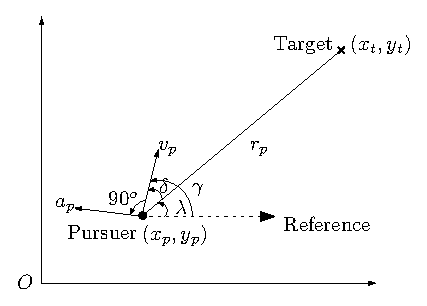
\includegraphics[scale=0.9, keepaspectratio]{Images/Eng_geom.eps}\\
				% \label{ChainLeader}
				% \caption{Engagement scenario against a stationary target.}
			\end{figure}
			
		\end{column}
	\end{columns}
		\begin{alertblock}{}
		%	 Given a pursuer's launch angle ($\gamma_p$), (constant) speed ($v_p$ ), initial range-to-go ($r_0$), and maximum lateral acceleration capability ($a_{\rm max}$), design a simple, easy-to-implement guidance law that meets the desired impact/approach angle ($\zeta$).
		\textcolor{blue}{\textbf{Objective: }\\
			Design a simple and easy-to-implement guidance law to satisfy the impact angle constraint}
	\end{alertblock}	
\end{frame}
%%%%%%%%%%%%%%%%%%%%%%%%%%%%%%%%%%%%%%%%%%%%%%%%%%%%%
\begin{comment}

\begin{frame}{Introduction: Why Impact Angle Constraints Are Important?}
	\begin{columns}
		\hspace*{0.2cm}
		\begin{column}{0.5\textwidth}
			\begin{defi}[Impact Angle]
				\begin{itemize}
					\item The angle between the velocity vectors of the two adversaries (target and interceptor) at the instant when interception of the target by the interceptor occurs. 
					\item For stationary targets, the impact angle is defined as the angle between the interceptor's velocity vector and some well-defined reference.
				\end{itemize}
			\end{defi}
		\end{column}
		\begin{column}{0.5\textwidth}
			\begin{figure}
				\centering
				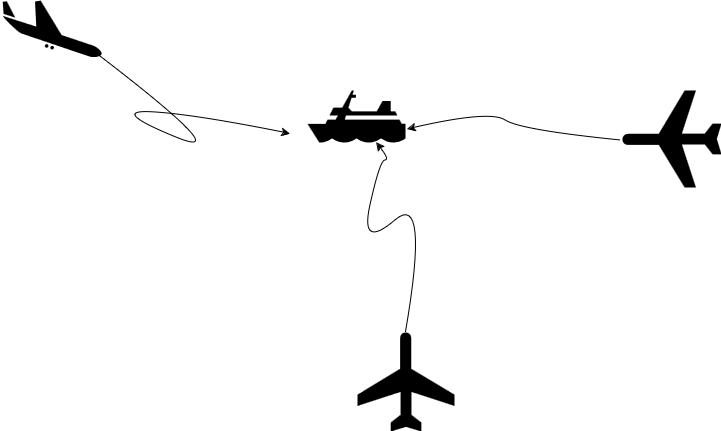
\includegraphics[scale=0.25]{Images/basicattack.png}
			\end{figure}
		\end{column}
	\end{columns}
	\vspace{0.5cm}
	\begin{columns}[T]
		\begin{column}{0.59\textwidth}
			%\column{0.46\textwidth}
			-- Exploit the geometric vulnerability\\    
			-- Enhancing warhead effectiveness \\
			-- Exploit fan-shaped coverage zones of radars
		\end{column}
		\vrule{}
		\begin{column}{0.41\textwidth}
			%\column{0.5\textwidth}
			-- Counter defense systems \\
			-- Improve hit-to-kill probability 
		\end{column}
	\end{columns}
\end{frame}


%%%%%%%%%%%%%%%%%%%%%%%%%%%%%%%%%%%%%%%%%%%%%%%%%%%%%
\begin{frame}{Literature Survey}
	\vspace{-0.2cm}
\begin{block}{Well Known Geometric Rules}
	\begin{enumerate}
		\item Pure Pursuit (PP), Deviated Pure Pursuit (DPP) or Proportional Navigation Guidance (PNG): In general does not enforce impact angle. Modified PNG, although enforce the impact angle but same as others requires high terminal acceleration. 
		\item  Polynomial Guidance : The entire path needs to be calculated in the beginning and hence too rigid. 
		\item Circular Navigation Guidance : Simple but Extremely Rigid Path
		\item Elliptic Guidance : Same as Circular, Simple but Rigid.
	\end{enumerate}
\end{block}
	\begin{block}{Spiral Based Laws ($r=\alpha\lambda^\beta$, where $\beta \in (0,1], \alpha \in \mathbb{R}$)}
		\begin{enumerate}
			\item T. Tripathi \& T. Shima [2019]~\footnotemark[1]  : Proposed a geometric rule based on Archimedean spiral ($\beta = 1$) $r(\lambda) = \alpha \lambda$. The geometric rule proposed was $\rm tan (\delta_p) = \lambda_p - \zeta$, where $\zeta$ is the desired impact angle.
			\item K. Mishra \& D. Mukherjee \& S. R. Kumar [2024]~\footnotemark[2]  : Proposed a geometric rule based on generalized spiral $r(\lambda) = \alpha \lambda^\beta$. The geometric rule proposed was $\rm tan (\delta_p) = (\lambda_p - \zeta) / \beta$.
		\end{enumerate}
	\end{block}
	\footnotetext[1]{\textcolor{blue}{Tripathy, T., \& Shima, T. (2019). Archimedean spiral-based intercept angle guidance. Journal of Guidance, Control, and Dynamics, 42(5), 1105-1115.}}
	\footnotetext[2]{\textcolor{blue}{Mishra, K., Mukherjee, D., \& Kumar, S. R. (2024, July). Spiral-based Guidance Strategy for Interception of Stationary Targets. In 2024 American Control Conference (ACC) (pp. 797-802). IEEE.}}
\end{frame}
\end{comment}
%%%%%%%%%%%%%%%%%%%%%%%%%%%%%%%%%%%%%%%%%%%%%%%%%%%%%
\begin{frame}{Curvature Vs Alpha}
	\vspace{-0.2cm}
	\begin{block}{Problems with the proposed laws}
		\begin{itemize}
			\item The proposed laws are independent of the spiral parameter $\alpha$ and the parameter $\alpha = r_0 / (\lambda_0 - \zeta)^\beta$ depends on initial Launch Angle and the initial Radial distance. Both of which are not usually a parameter of choice. 
		\end{itemize}
	\end{block}
	\begin{columns}
		\begin{column}{0.45\textwidth}
			$\kappa=\frac{\theta^{1-\beta}(\beta^2+\beta+\theta^2)}{\alpha(\beta^2+\theta^2)^{1.5}}$,
			\vspace{0.1cm}
			$\kappa_{max}=\frac{(3\beta^2+1)^{0.5}+\beta-1}{\alpha((3\beta^2+1)^{0.5}-1-\beta^2)^{(\beta-1)/2}((3\beta^2+1)^{0.5}-1)^{1.5}}$
			\vspace{0.1cm}
			$\kappa_{max}=\frac{f(\beta)}{\alpha}$
			
			\vspace{0.2cm}
			The curvature as well as maximum curvature and hence the Latax ($a=v_p^2\kappa$) is inversely proportional to $\alpha$.
		\end{column}
		\begin{column}{0.54\textwidth}
			\begin{figure}
				\centering
				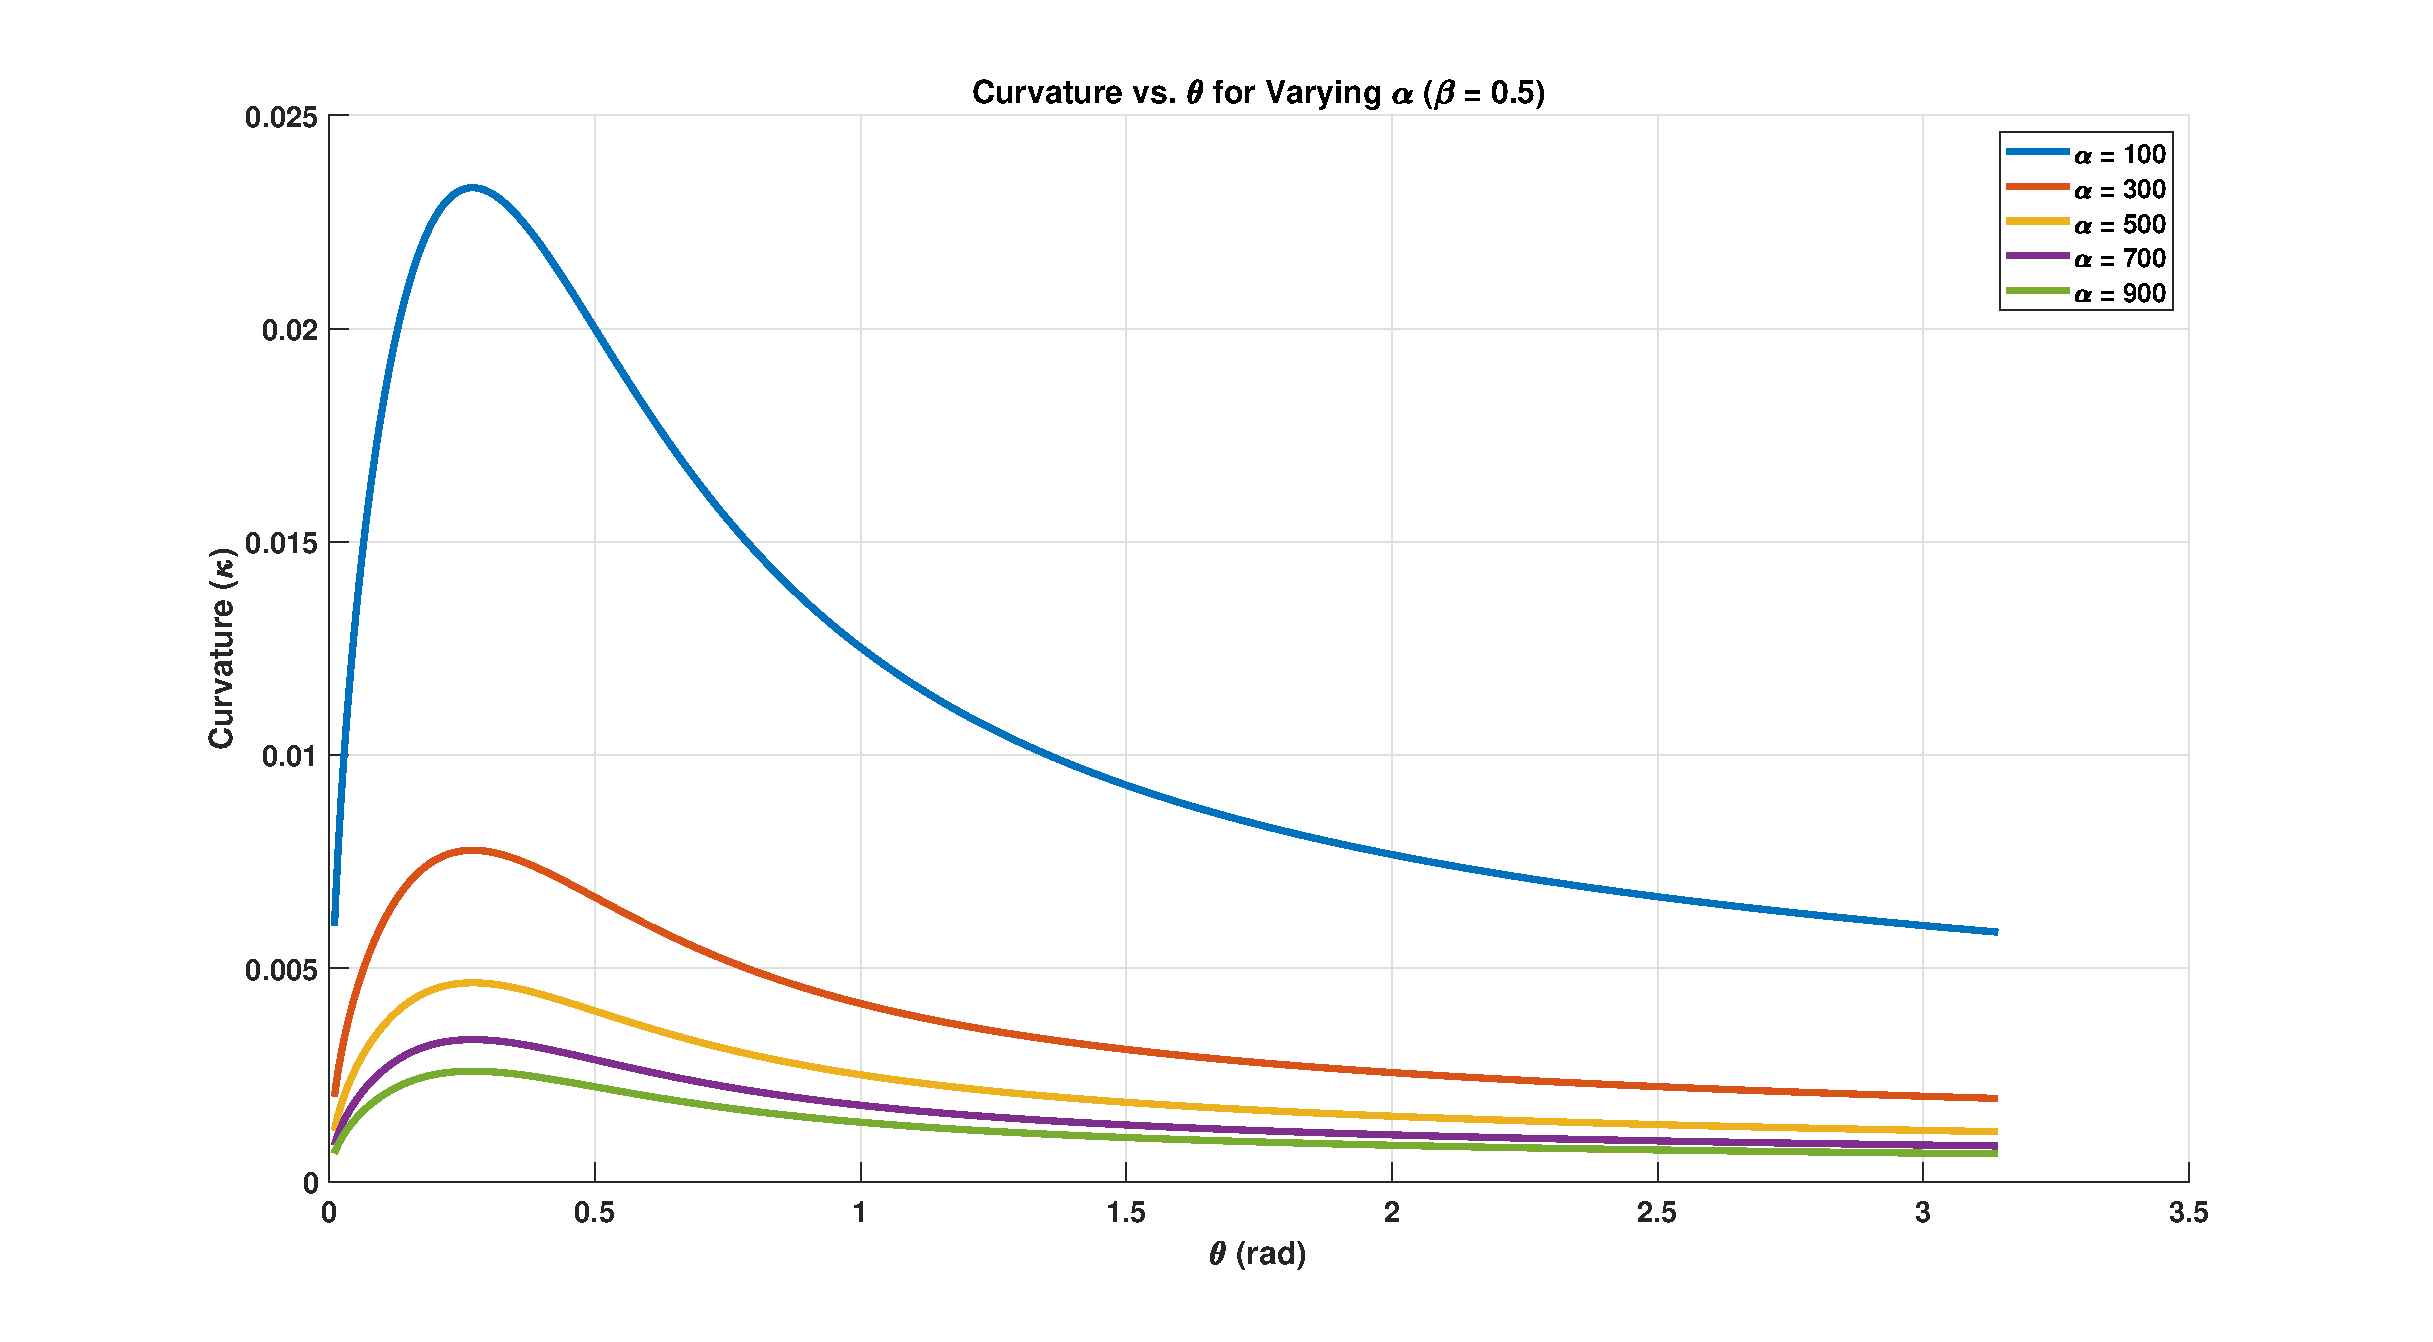
\includegraphics[scale=0.2]{Images/CurvVsAngle_FixedBeta_VaryingAlpha.eps}
			\end{figure}
		\end{column}
	\end{columns}
%	\vspace{-1.0 cm}
%\begin{columns}
%	\begin{column}{0.5\textwidth}
%		\begin{figure}
%			\centering
%			\includegraphics[scale=0.2]{CurvVsAngle_FixedAlpha_VaryingBeta.eps}
%		\end{figure}
%			The curvature as well as maximum curvature and hence the Latax is directly proportional to $\beta$ as shown.
%	\end{column}
%	\begin{column}{0.5\textwidth}
%	\end{column}
%\end{columns}
\end{frame}
%%%%%%%%%%%%%%%%%%%%%%%%%%%%%%%%%%%%%%%%%%%%%%%%%%%%%
\begin{frame}{Problem Demonstration}
	\vspace{-0.2cm}
	\begin{alertblock}{Inappropriate $\alpha$}
		If the initial value of $\alpha$ is not appropriate, the constrained lateral acceleration i.e. Latax (e.g. 30G) may not be sufficient to achieve the target. 
	\end{alertblock}
	The plot below reproduce the example demonstrated in the paper by K. Mishra \& D. Mukherjee \& S.R. Kumar~\footnotemark[1] by applying the constrained Latax.
	\vspace{-0.7cm} 
	\begin{columns}
		\begin{column}{0.5\textwidth}
			\begin{figure}
				\centering
				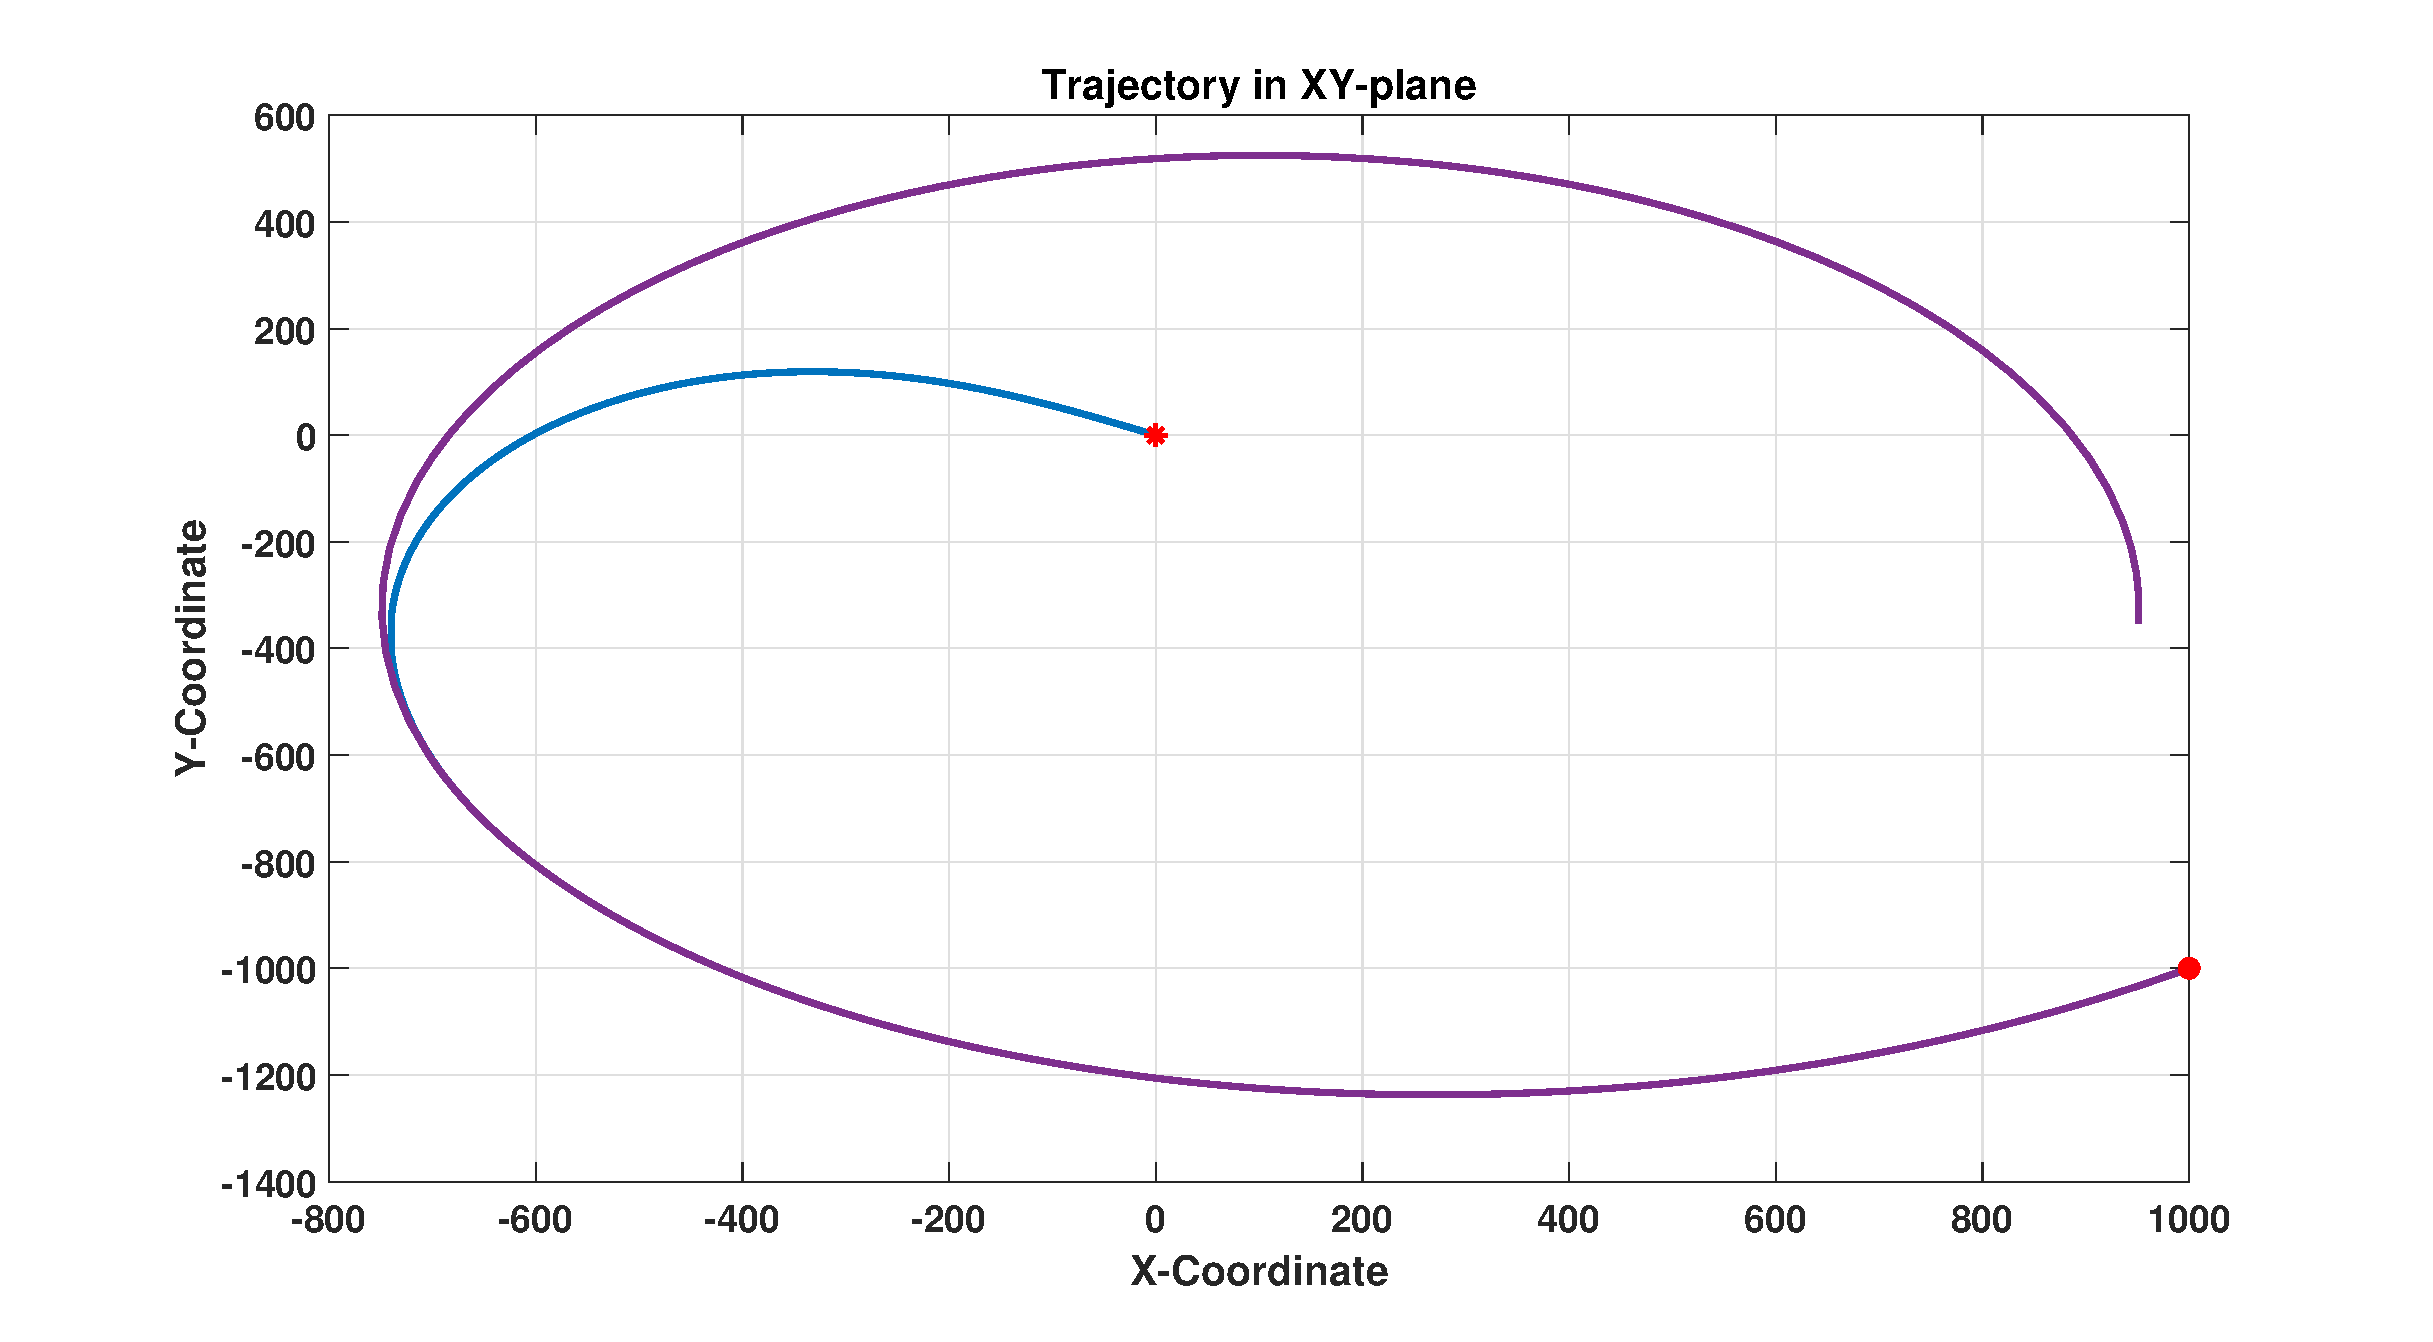
\includegraphics[scale=0.2]{Images/Trajectory_Kushagra.eps}
			\end{figure}
		\end{column}
		\begin{column}{0.5\textwidth}
			\begin{figure}
				\centering
				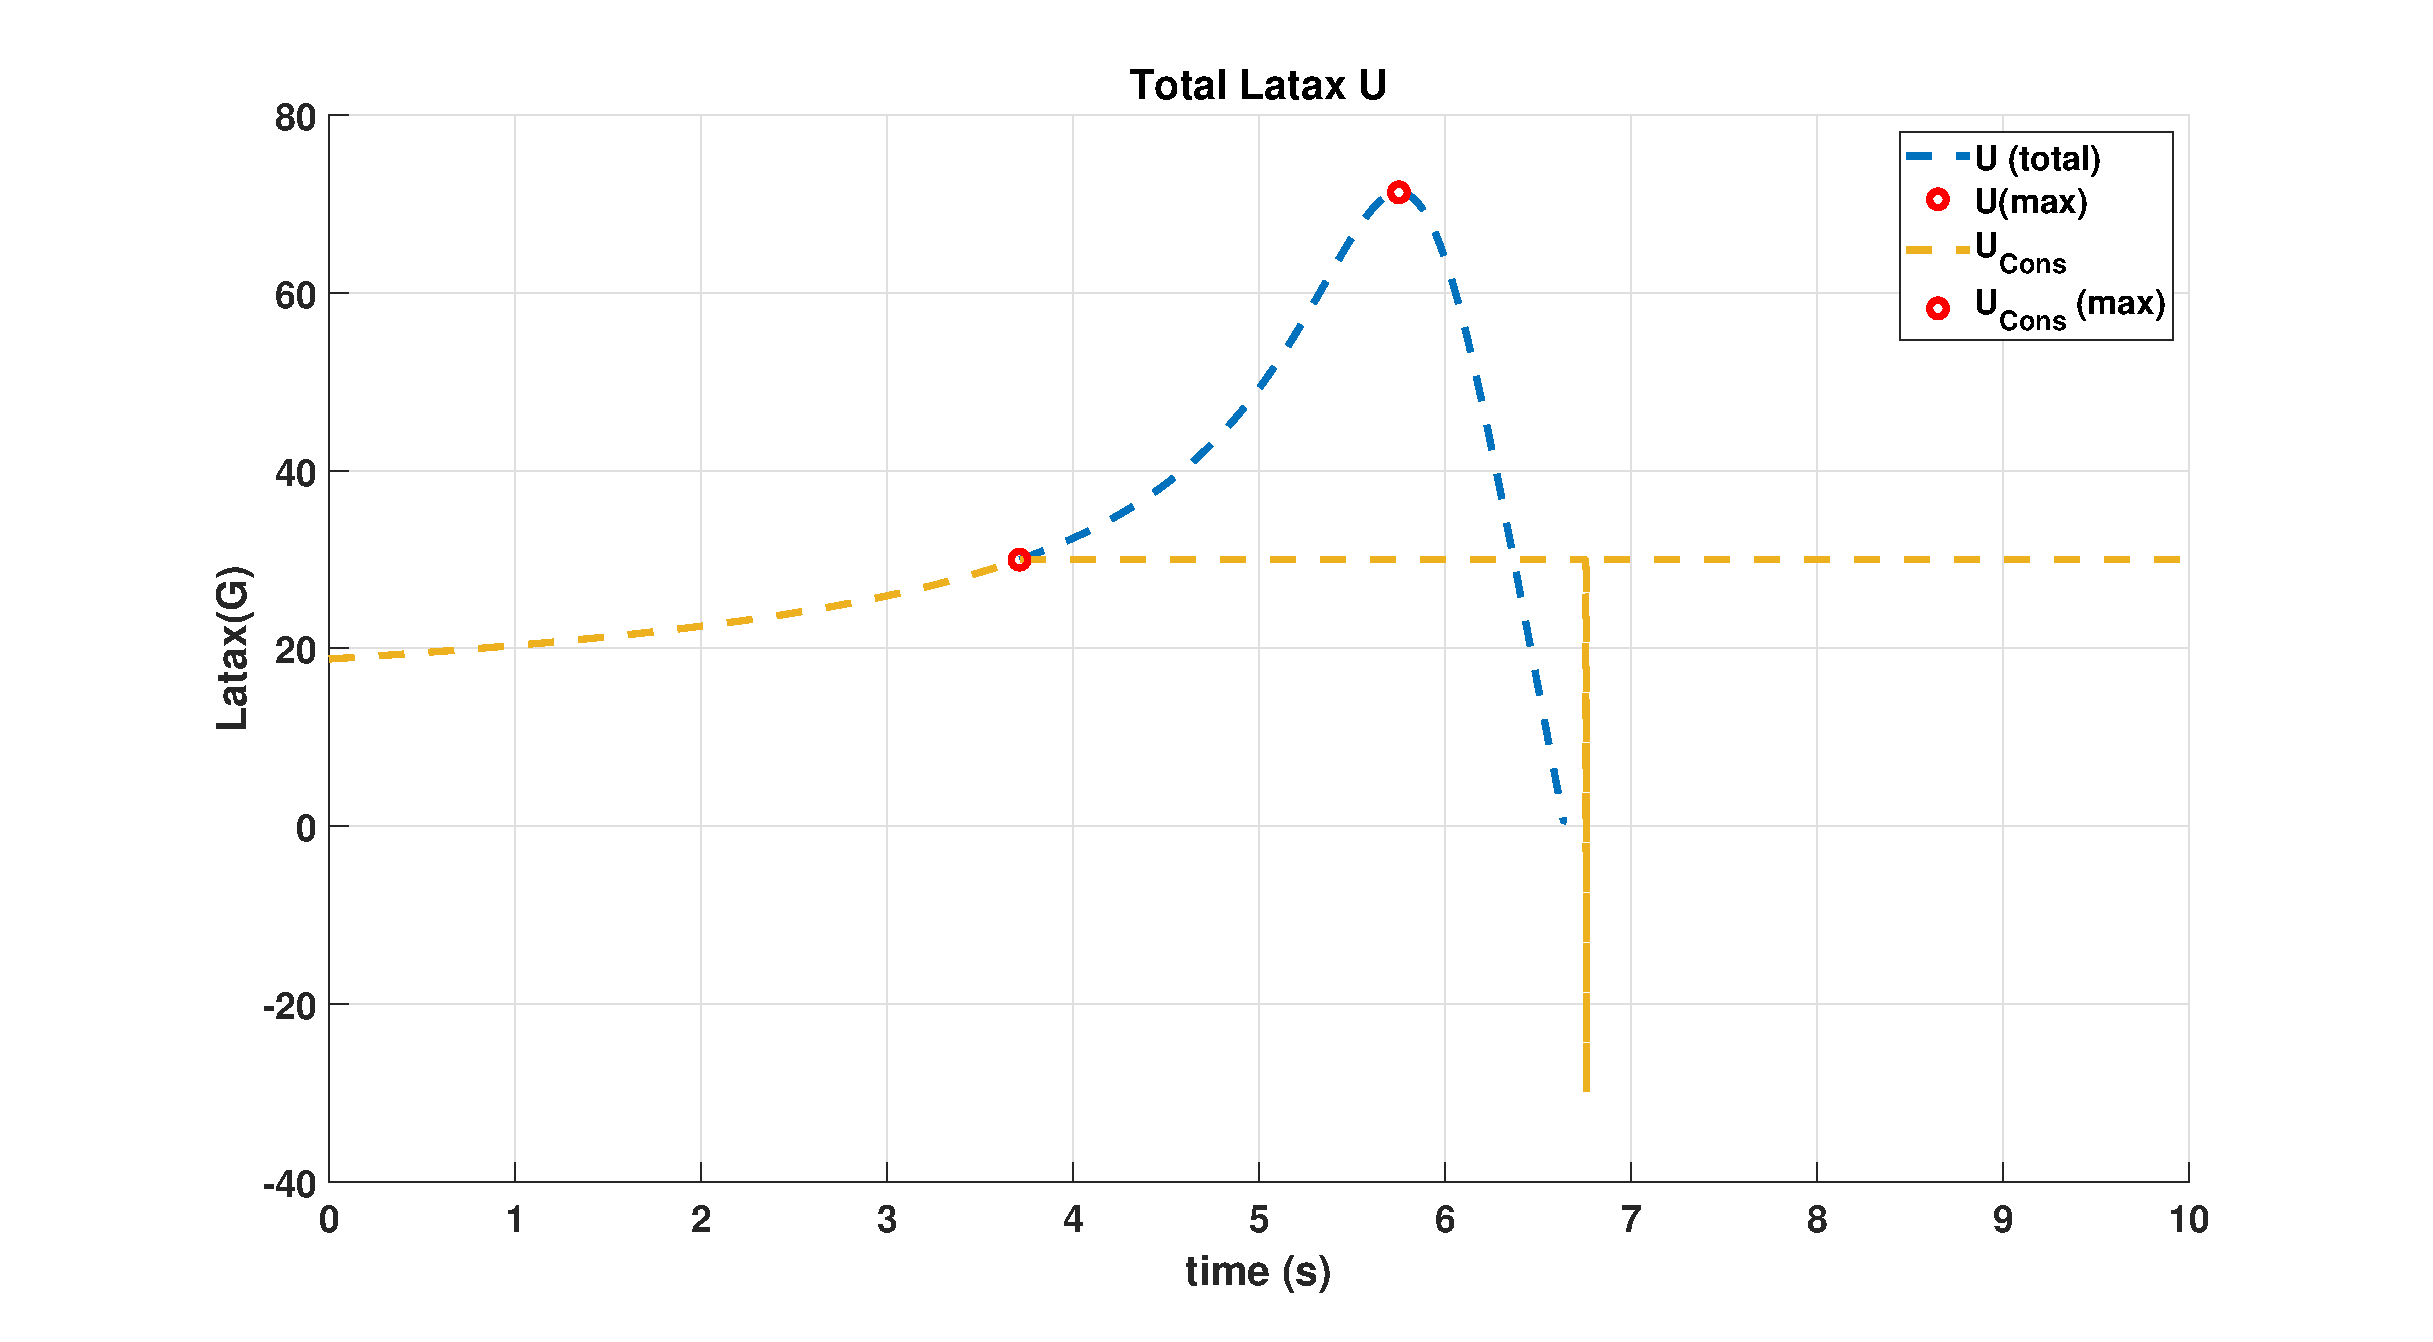
\includegraphics[scale=0.2]{Images/Latax_Kushagra.eps}
			\end{figure}
		\end{column}
	\end{columns}
\footnotetext[1]{\textcolor{blue}{Mishra, K., Mukherjee, D., \& Kumar, S. R. (2024, July). Spiral-based Guidance Strategy for Interception of Stationary Targets. In 2024 American Control Conference (ACC) (pp. 797-802). IEEE.}}
\end{frame}
%%%%%%%%%%%%%%%%%%%%%%%%%%%%%%%%%%%%%%%%%%%%%%%%%%%%%
\begin{frame}
		\begin{block}{Advantages of Spiral Based Trajectories}
		\begin{itemize}
			\item Direct Impact Angle Control : The geometry of the spiral is directly linked to the final impact angle.
			\item Curvature Constrained Path : Latax required by the pursuer throughout the engagement remains bounded.
			\item Terminal Acceleration : The terminal curvature ($\kappa$) and thus the terminal acceleration ($a$) tends to zero as $\lambda \rightarrow \zeta$.  
		\end{itemize}
	\end{block}
	\begin{myblock}{Two Stage Adaptive Law}
		We propose to use a geometric rule based on generalized spirals, $r(\alpha,\lambda) = \alpha (\lambda - \zeta)^\beta$.
		
		We introduce a two-stage Adaptive Control Technique to achieve the desired impact angle with the constrained Latax. 
		
		\textbf{Phase 1:} Feasibility Seeking : Calculate $\alpha_{ref} = \frac{v_p^2f(\beta)}{a_{max}}$. If $\alpha_0 < \alpha_{ref}$, then, drive the $\alpha$ to $\alpha_{ref}$. Otherwise, proceed directly with phase 2.\\
		\vspace{0.2cm}
		\textbf{Phase 2:} Terminal Guidance : We make $\dot{\alpha}=0$. Phase 1 already ensured that Constrained Latax is sufficient to drive the pursuer to the target.
	\end{myblock}
\end{frame}
%%%%%%%%%%%%%%%%%%%%%%%%%%%%%%%%%%%%%%%%%%%%%%%%%%%%%
\begin{frame}{Guidance Law for Phase 1}
\begin{myblock}{Feasibility Seeking}
	Given the dynamics of the system as follows:
	$$\begin{bmatrix}
		\dot{r_p} \\ 
		\dot{\lambda_p} \\
		\dot{\gamma_p}
	\end{bmatrix}=\begin{bmatrix}
	-v_p \cos(\gamma_p-\lambda_p) \\ 
	\frac{-v_p \sin(\gamma_p-\lambda_p)}{r_p} \\
	(a_p+n)/v_p
	\end{bmatrix}=\begin{bmatrix}
	-v_p \cos(\delta_p) \\ 
	\frac{-v_p \sin(\delta_p)}{r_p} \\
	(a_p+n)/v_p
	\end{bmatrix}$$
	where, $\max(n)=N_0$ is assumed to be bounded uniformly distributed noise. We take \\
	$$e=e_{shape}+k_re_{scale}$$
	where, $e_{shape}=\delta_p-\tan^{-1}{(\frac{\lambda_p-\zeta}{\beta}}), ~~ e_{scale}= r-\alpha(\lambda_p-\zeta)^{\beta}$.
\end{myblock}
\end{frame}
%%%%%%%%%%%%%%%%%%%%%%%%%%%%%%%%%%%%%%%%%%%%%%%%%%%%%
\begin{frame}
%	\begin{myblock}{}
		$$\boxed{\dot{e} = \dot{e}_{shape}+k_r\dot{e}_{scale}}$$
		$\mathbf{\dot{e}_{shape}}=\frac{a_p+n}{v_p}+\frac{v_p\sin(\delta_p)}{r_p}(1+\frac{1}{\beta(1+(\lambda_p-\zeta)^2/\beta^2)}),\quad \mathbf{\dot{e}_{scale}}=-v_p\cos(\delta_p)+\frac{v_p\sin(\delta_p)\alpha\beta(\lambda_p-\zeta)^{\beta-1}}{r_p}-\dot{\alpha}(\lambda_p-\zeta)^\beta$
		
		\vspace{0.2cm}
		Choosing,
		\begin{align*}
		a_{p} =& \color{magenta}{\underbrace{-\frac{v_p^2\sin(\delta_p)}{r_p}(1+\frac{1}{\beta(1+(\lambda_p-\zeta)^2/\beta^2)})}_{a_{shape}}}+\color{blue}{\underbrace{k_r(v_p^2\cos(\delta_p)-\frac{v_p^2\sin(\delta_p)\alpha\beta(\lambda_p-\zeta)^{\beta-1}}{r_p}+v_p\dot{\alpha}(\lambda_p-\zeta)^\beta)}_{a_{scale}}}\\
		&\color{teal}{+\underbrace{(\frac{c_1|e|^{\alpha_1}}{\tau^{\mu_1}}+\frac{c_2|e|^{\alpha_2}}{\tau^{\mu_2}})sgn(e)}_{a_{uncertain}}}	
		\end{align*}
		
	where $c_1,c_2,\mu_1,\mu_2 \in \mathbb{R} > 0,~~ \alpha_1 \in (0,1),~~ \alpha_2 > 1, ~~ \tau = T^*-t$
		
%	\end{myblock}
\begin{block}{}
		Appropriate values of the controller parameters and a proportional control for $\dot{\alpha}=K_p(\alpha_{ref}-\alpha(t))$, achieve the feasible trajectory. 
\end{block}
\end{frame}
%%%%%%%%%%%%%%%%%%%%%%%%%%%%%%%%%%%%%%%%%%%%%%%%%%%%%
\begin{frame}{Guidance Law for Phase 2}
	\begin{myblock}{Terminal Guidance}
		We take $\boxed{\dot{\alpha}=0}$ for this phase. Thus, $$\dot{e}_{scale}=-v_p\cos(\delta_p)+\frac{v_p\sin(\delta_p)\alpha\beta(\lambda_p-\zeta)^{\beta-1}}{r_p}$$
		
		Making $\dot{e}_{scale}=0$, 
		$$ \tan \delta_p = \frac{(\lambda - \zeta)}{\beta} \implies e_{shape}=0$$
		Therefore, $e_{scale}$ and $e_{shape}$ converges to the same geometric law as mentioned in the earlier paper\footnotemark[1].
	\end{myblock}
	\footnotetext[1]{\textcolor{blue}{Mishra, K., Mukherjee, D., \& Kumar, S. R. (2024, July). Spiral-based Guidance Strategy for Interception of Stationary Targets. In 2024 American Control Conference (ACC) (pp. 797-802). IEEE.}}
\end{frame}
%%%%%%%%%%%%%%%%%%%%%%%%%%%%%%%%%%%%%%%%%%%%%%%%%%%%%
\begin{frame}{Simulation Parameters}
\begin{itemize}
	\item Pursuer Position: $ x_p(0) = 1000 \text{ m};~~ y_p(0) = -1000 \text{ m}$
	\item Target Position: $x_t(0) = 0 \text{ m};~~y_t(0) = 0 \text{ m}$
	\item Pursuer's Constant Velocity: $v_p = 500 \text{ m/s}$
	\item Lead Angle: $\delta_p(0) = \pi/6$
	\item Desired Impact Angle: $\zeta = -\pi/4$
	\item Maximum Acceleration: $a_{max} = 30*9.8 \text{ m/$s^2$}= 30G \text{ m/$s^2$}$
	\item Fixed Spiral Parameter : $\beta = 0.5$
	\item Initial Spiral Parameter : $r_p(0) = 1414.2 \text{ m}, ~~ \alpha(0)=797.8846, ~~ \lambda(0)= 3 \pi/4$
\end{itemize}
	
\end{frame}
%%%%%%%%%%%%%%%%%%%%%%%%%%%%%%%%%%%%%%%%%%%%%%%%%%%%%
\begin{frame}{Trajectory Vs Time}
	%\vspace{-1.0cm}
	\begin{figure}
		\centering
		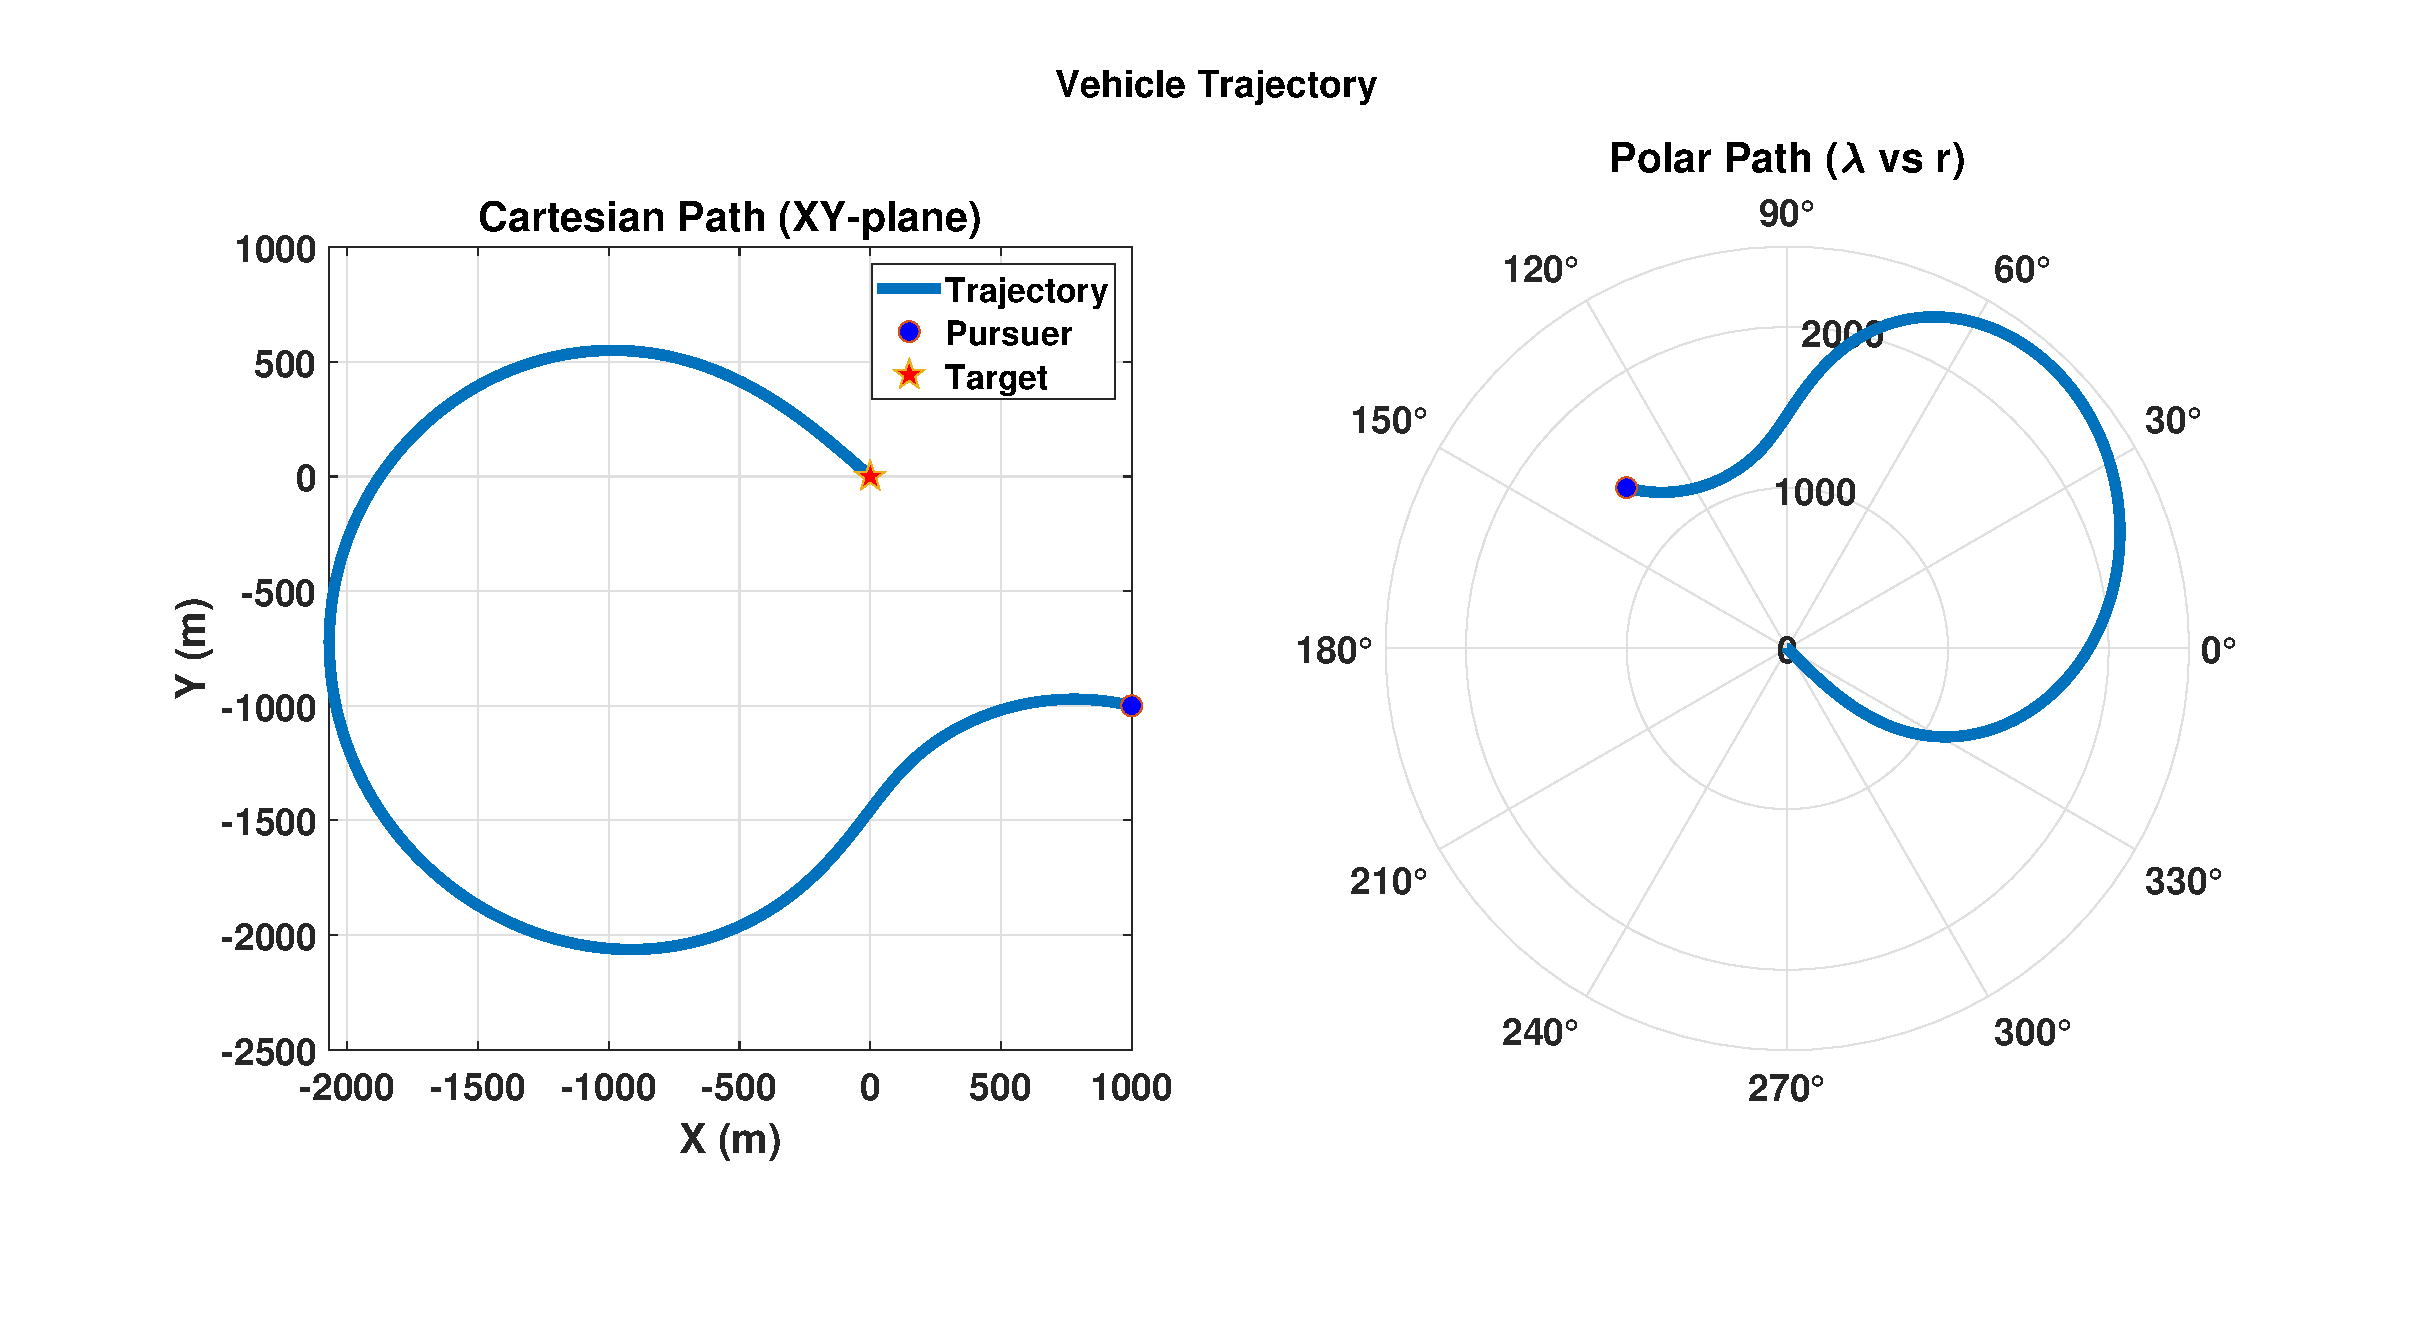
\includegraphics[scale=0.35]{Images/VehicleTrajectory.eps}
	\end{figure}
\end{frame}
%%%%%%%%%%%%%%%%%%%%%%%%%%%%%%%%%%%%%%%%%%%%%%%%%%%%%
\begin{frame}{States vs Time}
	\vspace{-0.3cm}
	\begin{figure}
		\centering
		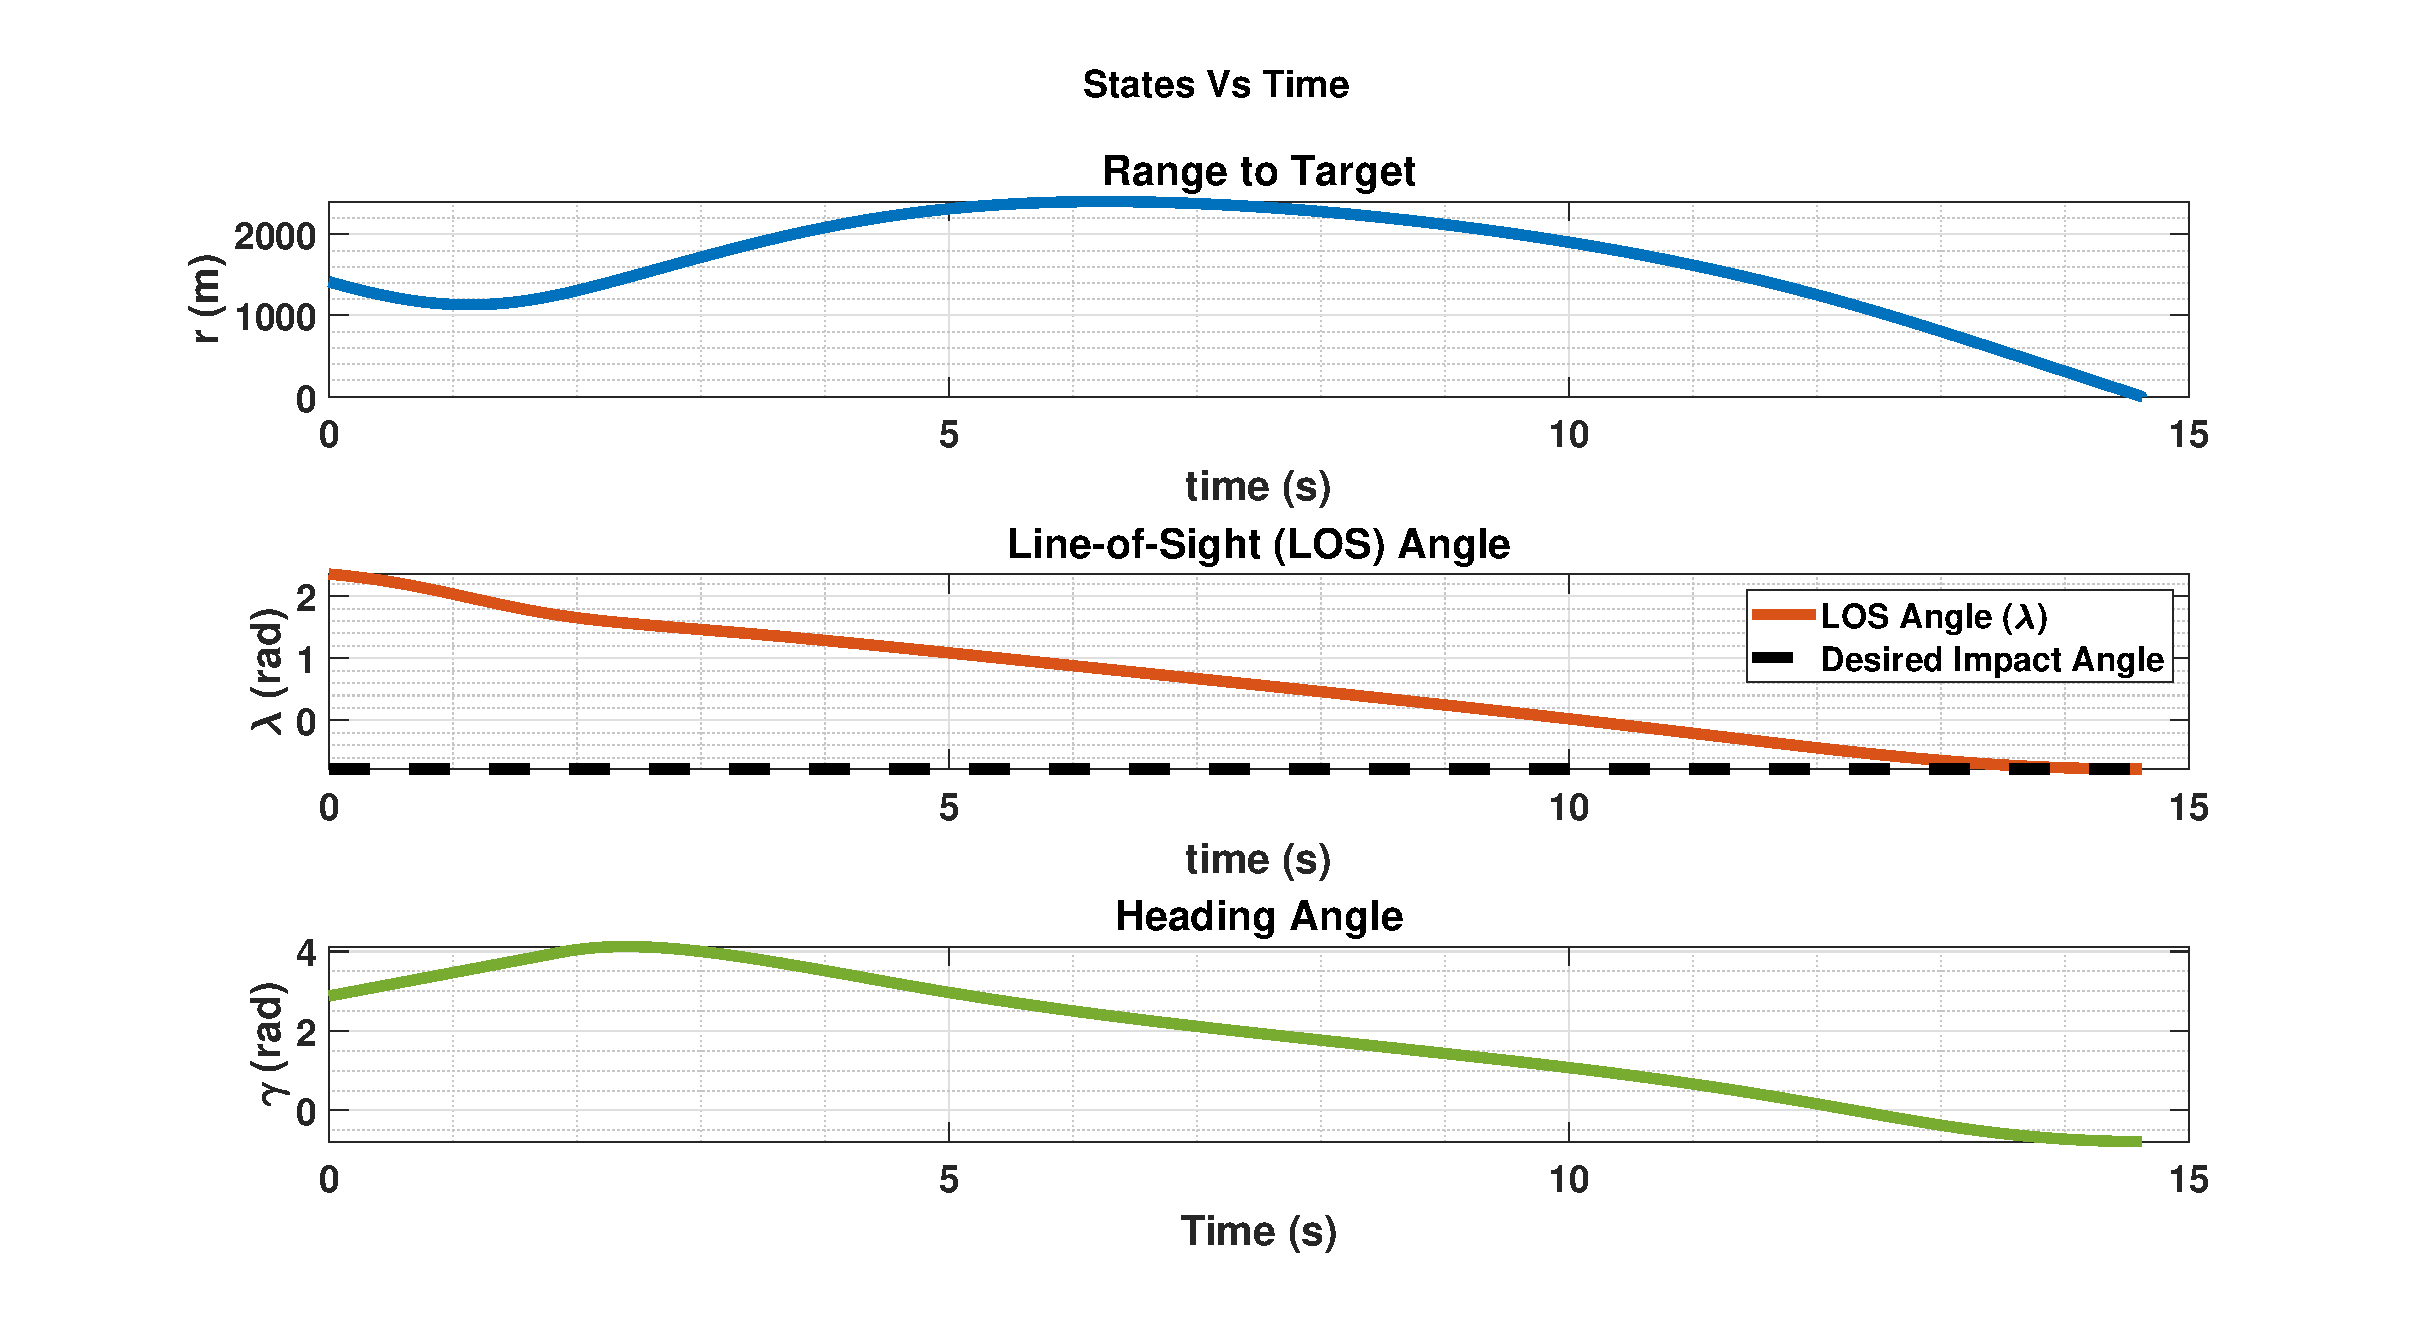
\includegraphics[scale=0.35]{Images/StatesVsTime.eps}
	\end{figure}
\end{frame}
%%%%%%%%%%%%%%%%%%%%%%%%%%%%%%%%%%%%%%%%%%%%%%%%%%%%%
\begin{frame}{Latax Commanded vs Actual}
	\vspace{-0.3cm}
		\begin{figure}
		\centering
		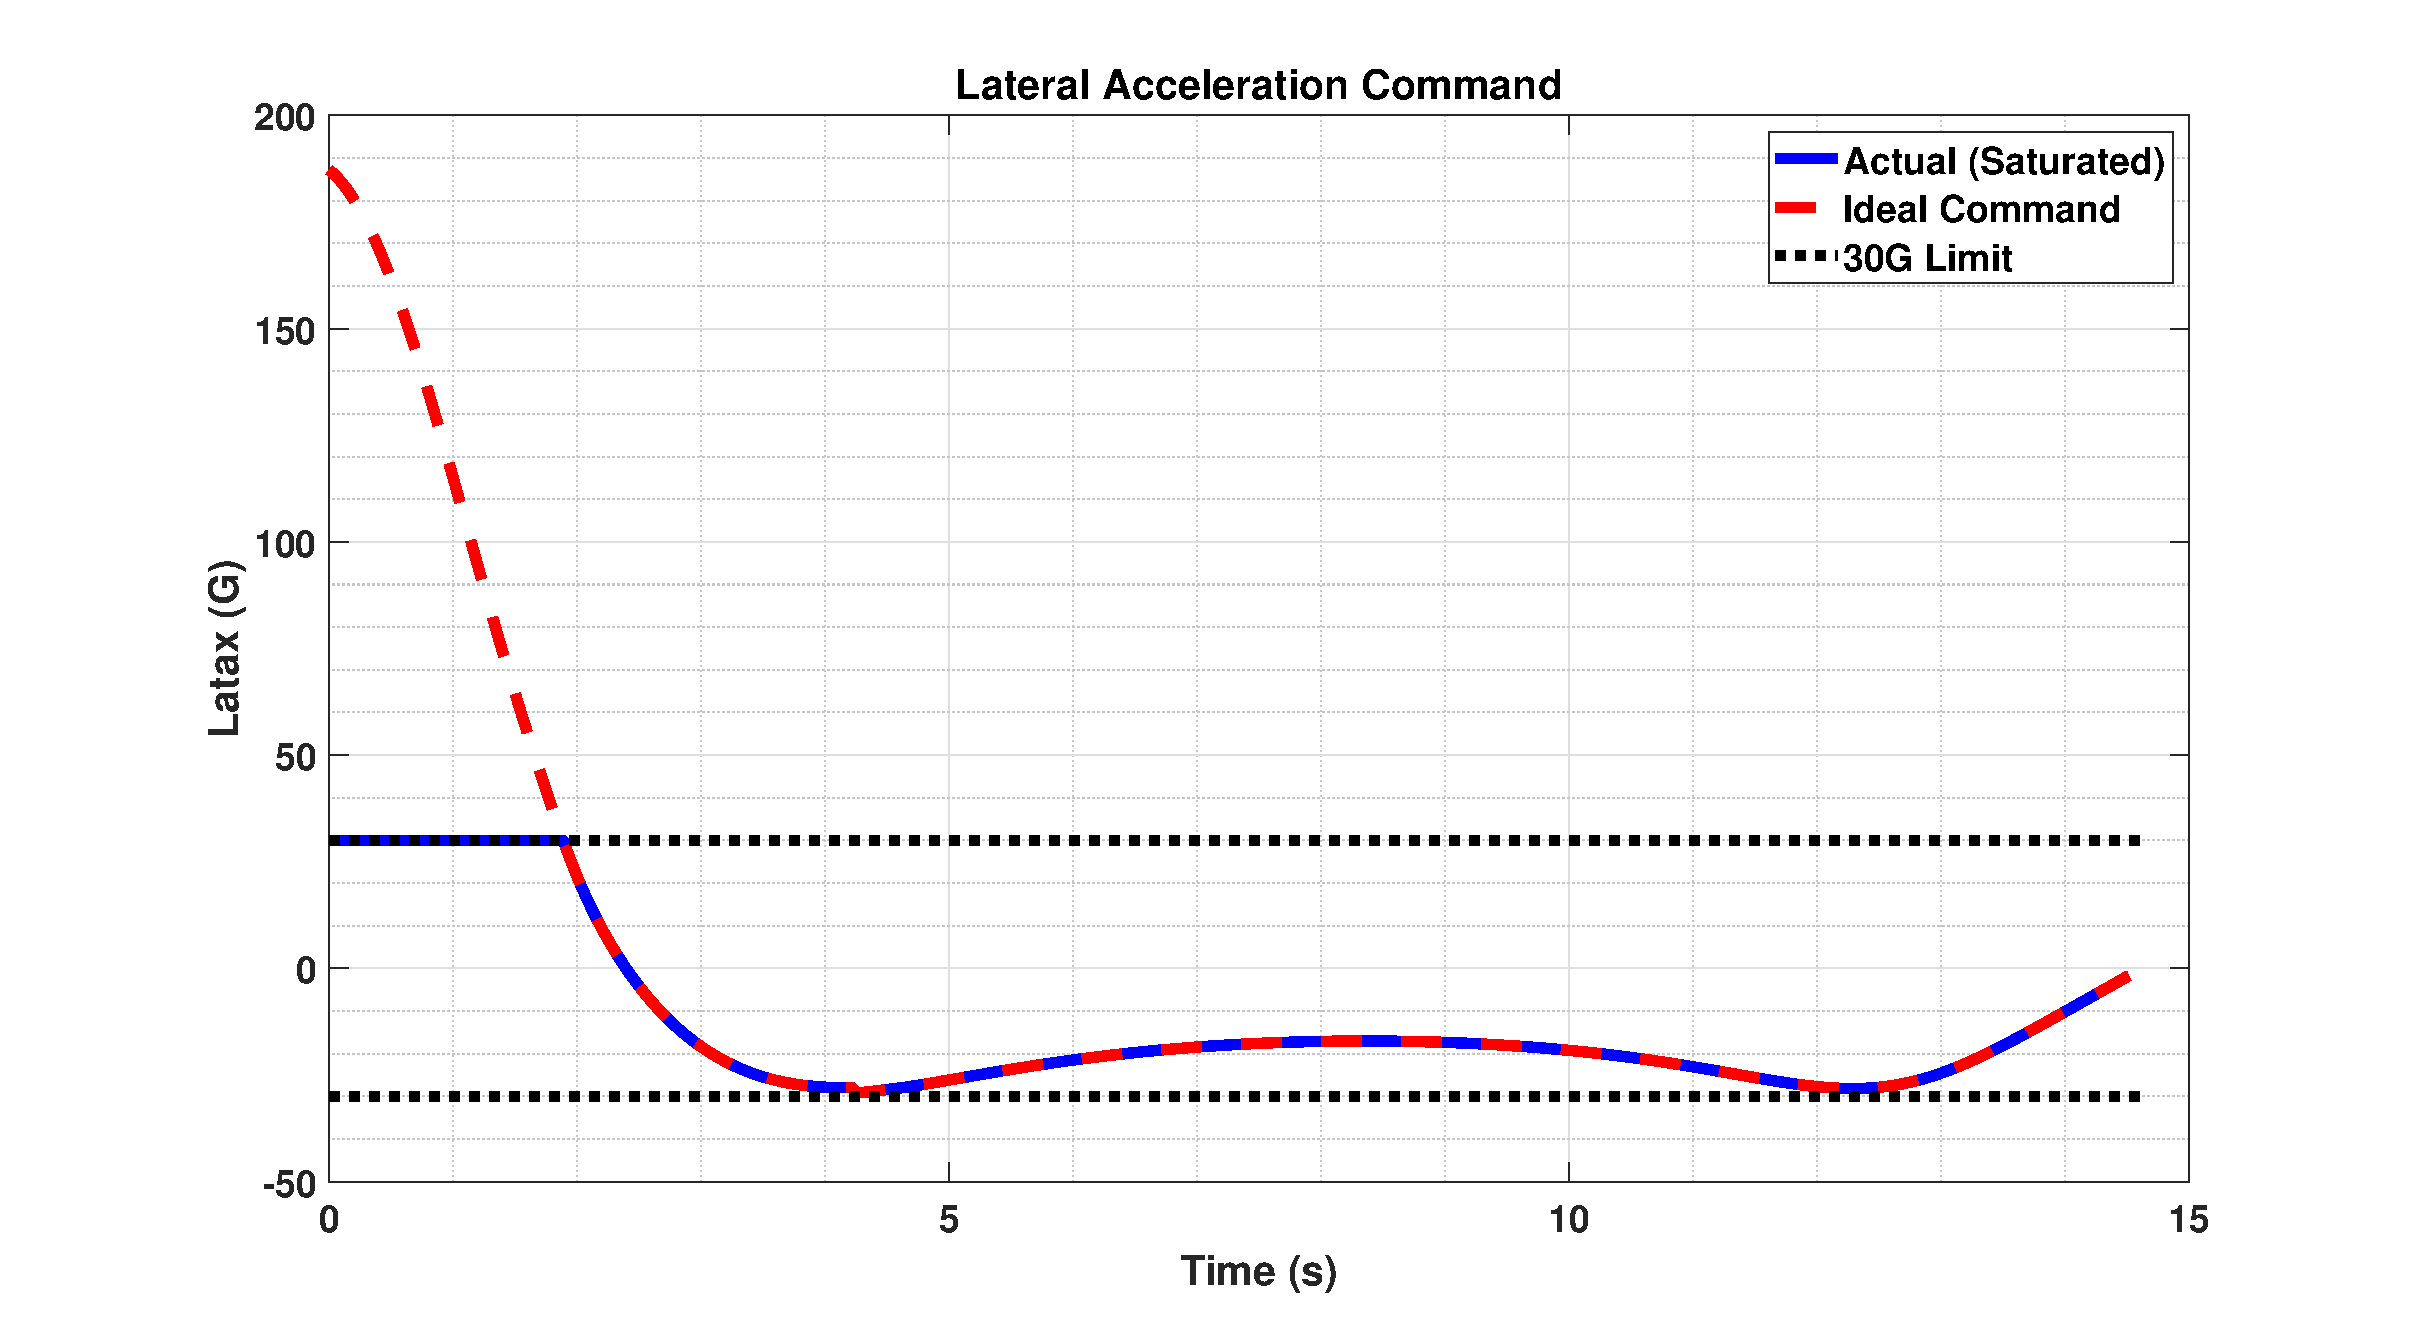
\includegraphics[scale=0.3]{Images/LATAX_ActualVsIdeal.eps}
	\end{figure}
\end{frame}
%%%%%%%%%%%%%%%%%%%%%%%%%%%%%%%%%%%%%%%%%%%%%%%%%%%%%
\begin{frame}{Shape and Scale Input}\label{Control}
	\vspace{-0.3cm}
		\begin{figure}
		\centering
		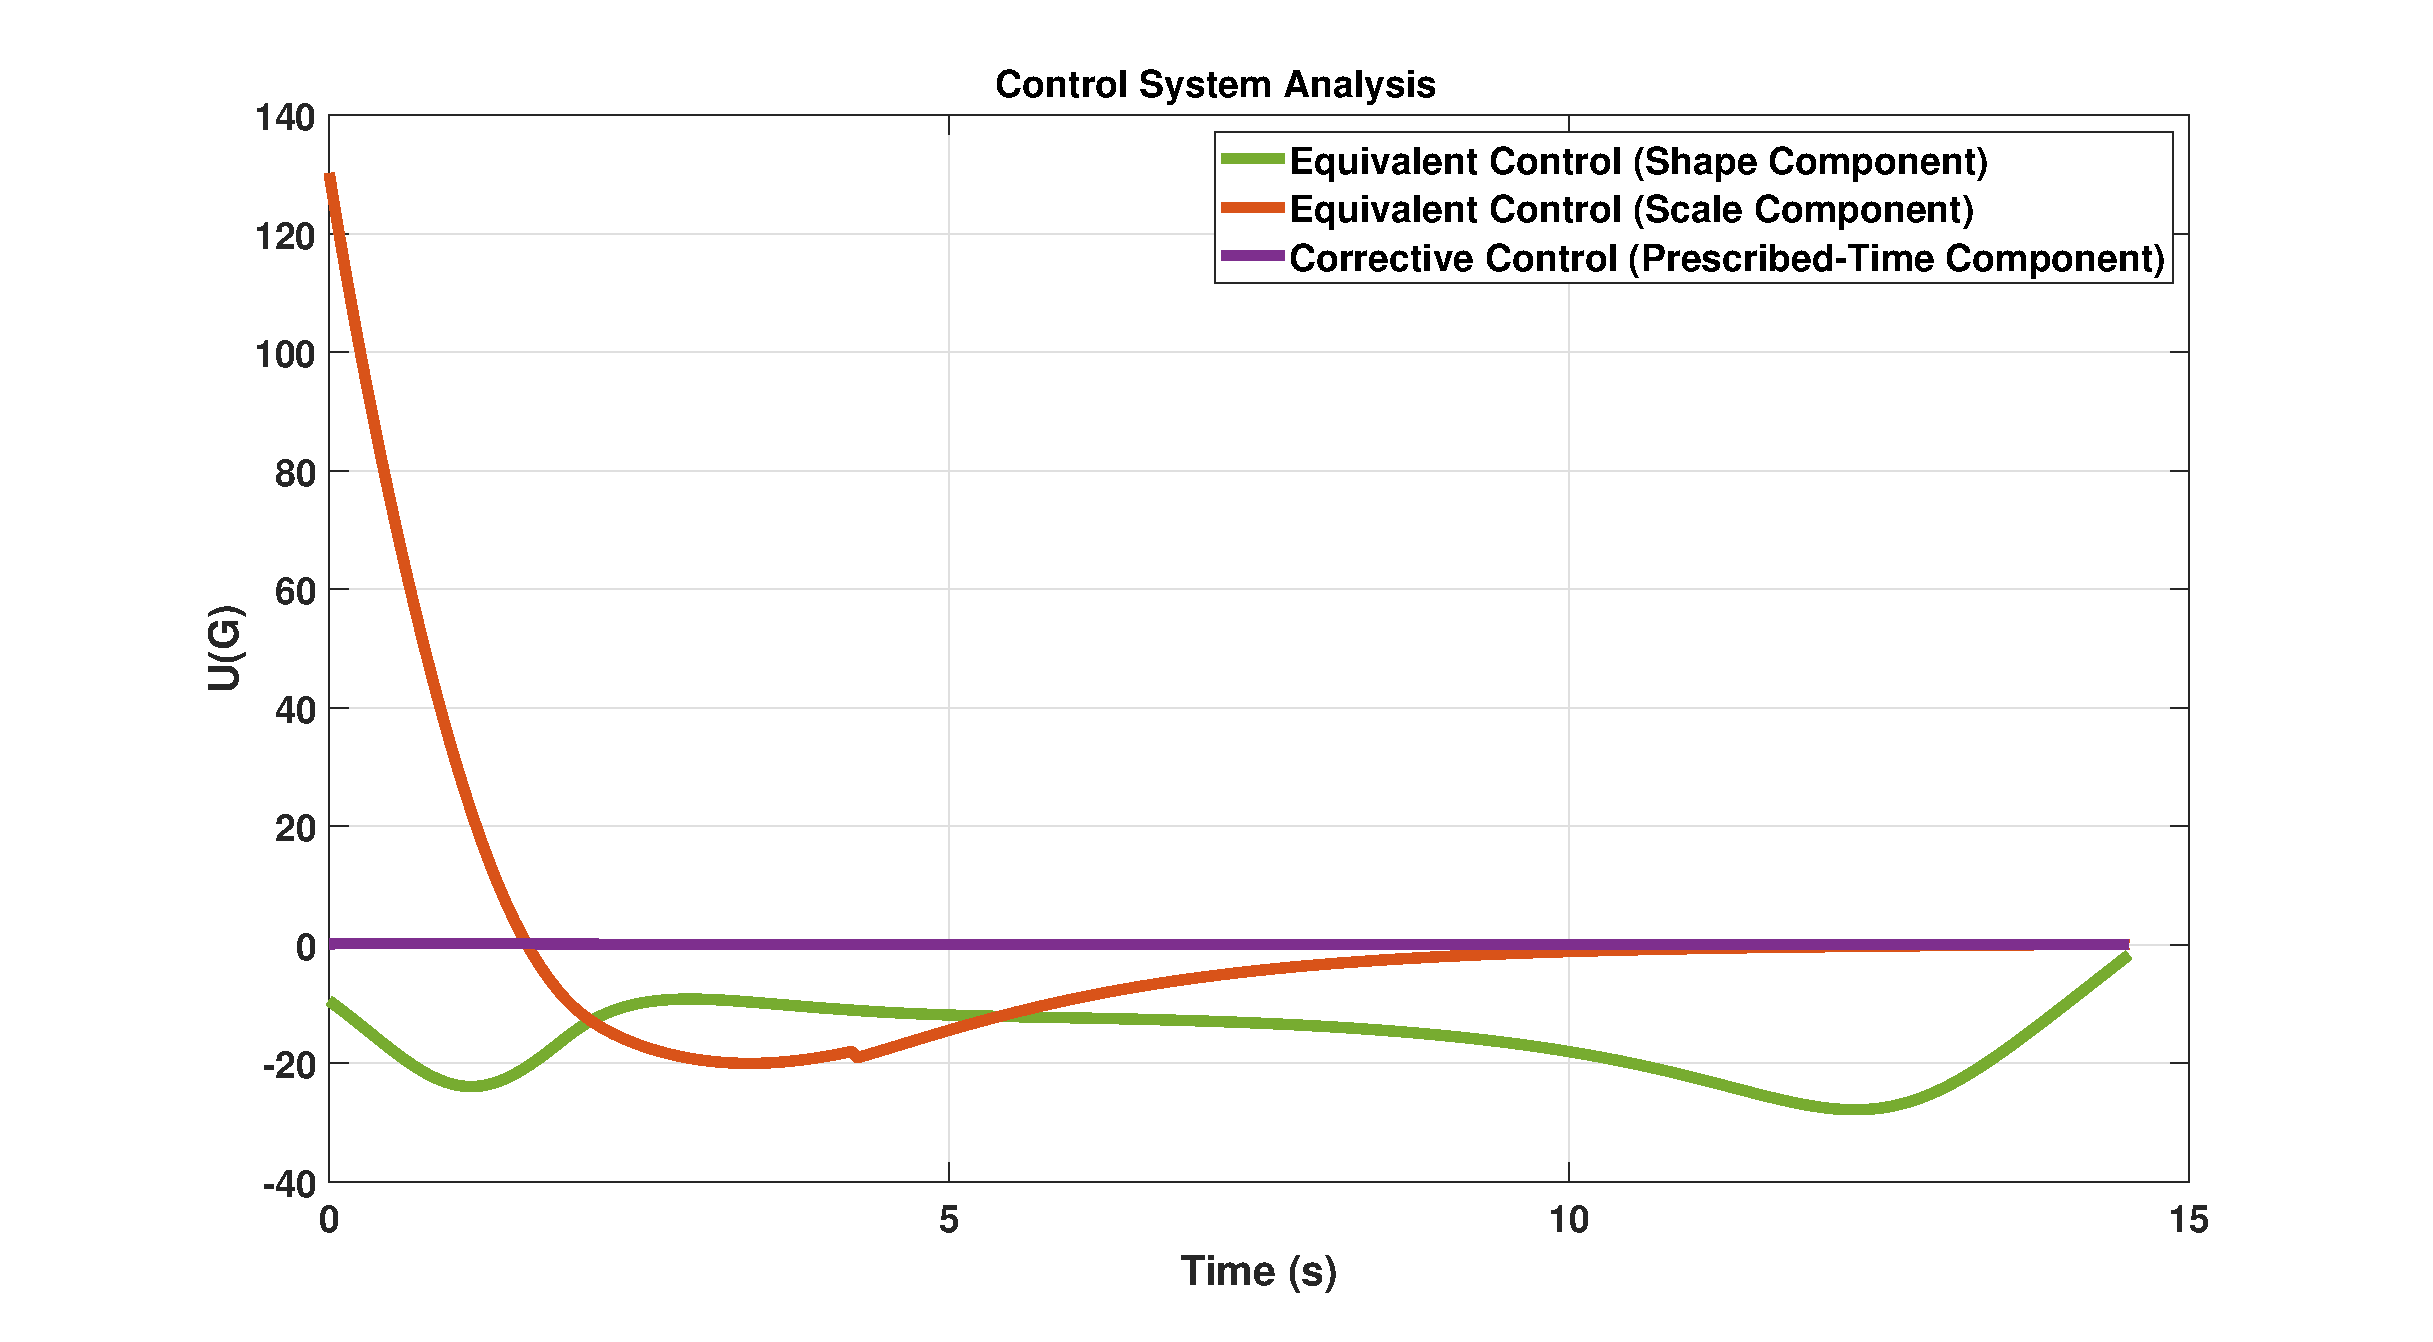
\includegraphics[scale=0.3]{Images/Control_Shape_Scale_PT.eps}
	\end{figure}
	\hyperlink{Corr}{\beamerbutton{PT Control}}
\end{frame}
%%%%%%%%%%%%%%%%%%%%%%%%%%%%%%%%%%%%%%%%%%%%%%%%%%%%%
\begin{frame}{Multi-Agent Extension}
	\begin{block}{Operational Motivation}
		\begin{itemize}
			\item Attack from a specified \textbf{sector} instead of a single direction.
			\item Make System Scalable
			\item Maintain actuator constraint ($a_{max} = 30G$) for all agents.
		\end{itemize}
	\end{block}
	
	\begin{alertblock}{New Challenges}
		\begin{itemize}
			\item Each agent has different initial condition.
			\item Initial Spiral parameter $\alpha_i$ differs for each agent.
			\item Spiral Parameters and Desired Impact Angle both affect the $\alpha_{req}$ for smoother trajectory.  
		\end{itemize}
	\end{alertblock}
\end{frame}
%%%%%%%%%%%%%%%%%%%%%%%%%%%%%%%%%%%%%%%%%%%%%%%%%%%%%
\begin{frame}{Multi-Agent Engagement Model}
	For $i = 1,2,\dots,N$
	\[
	\dot r_i = -v_p \cos(\delta_i)
	\]
	\[
	\dot \lambda_i = \frac{-v_p \sin(\delta_i)}{r_i}
	\]
	\[
	\dot \gamma_i = \frac{a_i}{v_p}
	\]
	
	\begin{block}{Impact Angle Sector Assignment}
		Impact angles distributed inside a sector:
		
		\[
		\zeta_i \in [\theta_{start},\theta_{end}]
		\]
		
		Uniform assignment:
		
		\[
		\zeta_i = \theta_{start} + \frac{i-1}{N-1}
		(\theta_{end}-\theta_{start})
		\]
	\end{block}
	
\end{frame}
%%%%%%%%%%%%%%%%%%%%%%%%%%%%%%%%%%%%%%%%%%%%%%%%%%%%%
\begin{frame}{Spiral Manifold for Each Agent}
	
	Each agent follows:
	
	\[
	r_i = \alpha_i (\lambda_i - \zeta_i)^{\beta_i}
	\]
	
	\begin{block}{Error Definition}
		\[
		e_i = e_{shape,i} + k_r e_{scale,i}
		\]
		
		\[
		e_{shape,i} = \delta_i - \tan^{-1}\left(\frac{\lambda_i - \zeta_i}{\beta_i}\right)
		\]
		
		\[
		e_{scale,i} = r_i - \alpha_i (\lambda_i - \zeta_i)^{\beta_i}
		\]
	\end{block}
	
	Each agent independently satisfies impact angle constraint.
\end{frame}
%%%%%%%%%%%%%%%%%%%%%%%%%%%%%%%%%%%%%%%%%%%%%%%%%%%%%
%%%%%%%%%%%%%%%%%%%%%%%%%%%%%%%%%%%%%%%%%%%%%%%%%%%%%
\begin{frame}{Two-Phase Multi-Agent Guidance}
We introduce coupling at the level of spiral scaling:

\[
\dot{\alpha}_i = -k_\alpha \sum_{j \in \mathcal{N}_i}
(\alpha_i - \alpha_j)
\]

\begin{block}{Leader-Follower Implementation}
	Leader:
	\[
	\alpha_1 \rightarrow \max(\alpha_{min,i})
	\]
	
	Followers:
	\[
	\dot{\alpha}_i = -k_\alpha (\alpha_i - \alpha_{parent})
	\]
\end{block}
	\begin{block}{Phase 1: Feasibility + Consensus}
		\begin{itemize}
			\item Compute $\alpha_{min,i}$
			\item Drive $\alpha_i \rightarrow \alpha_{ref}$
			%\item Apply prescribed-time control on $e_i$
			\item Maintain $|a_i| \le a_{max}$
		\end{itemize}
	\end{block}
\end{frame}
\begin{frame}	
	\begin{block}{Phase 2: Terminal Guidance}
		\begin{itemize}
			\item Freeze $\alpha_i$
			\item Enforce spiral manifold
			\item $\tan \delta_i = \frac{\lambda_i - \zeta_i}{\beta_i}$
			\item Terminal curvature $\rightarrow 0$
		\end{itemize}
	\end{block}
		Ensures:
	\begin{itemize}
		\item Topology is defined in a manner such that it is agnostic to link failures.
		\item Feasible curvature for all agents
		\item Coordinated spiral expansion
		\item Smooth scaling 
	\end{itemize}
\end{frame}
%%%%%%%%%%%%%%%%%%%%%%%%%%%%%%%%%%%%%%%%%%%%%%%%%%%%% 
\begin{frame}{Simulations}	
		N=4; x0 = [1000 1200 800 900]; y0 = [-1000 -900 -1100 -950];\\
		\begin{columns}
			\begin{column}{0.5\textwidth}
				\begin{figure}
					%\centering
					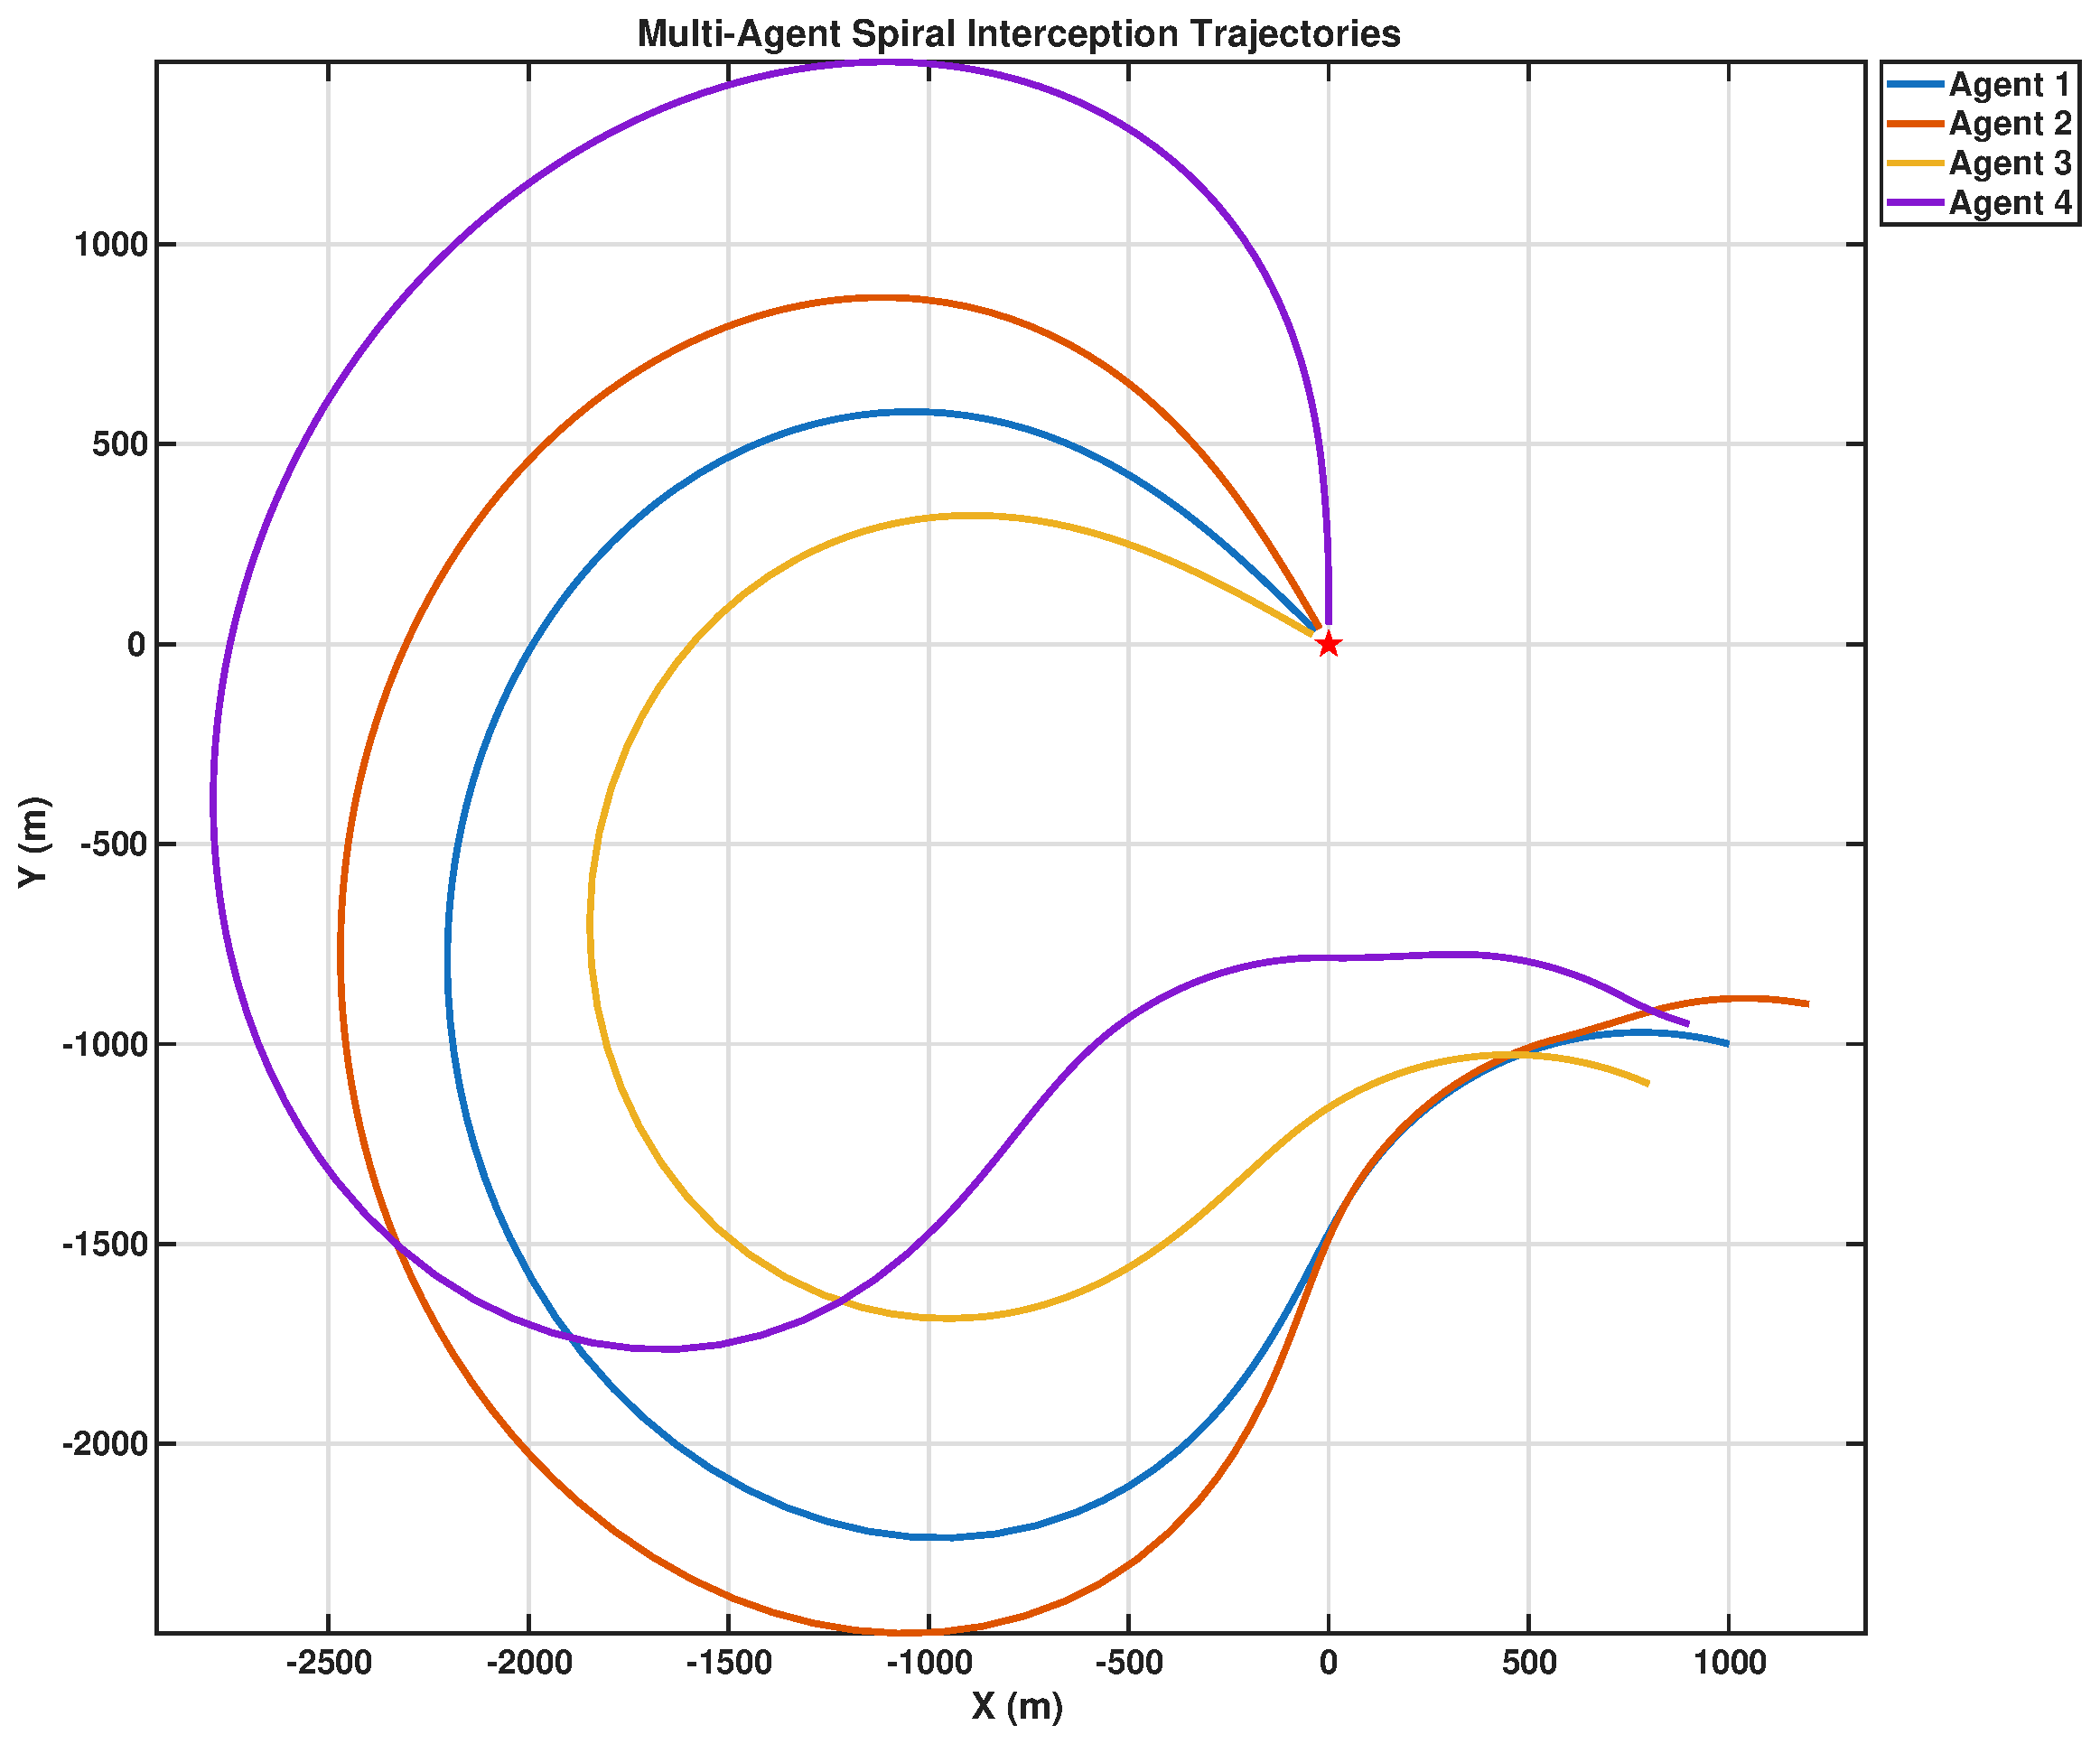
\includegraphics[scale=0.15]{Images/4Agent_Case1_Trajectory.eps}
					\caption{Trajectory of 4 Agents intercepting at different Impact Angle}
				\end{figure}
			\end{column}
			\begin{column}{0.5\textwidth}
				\begin{figure}
					%\centering
					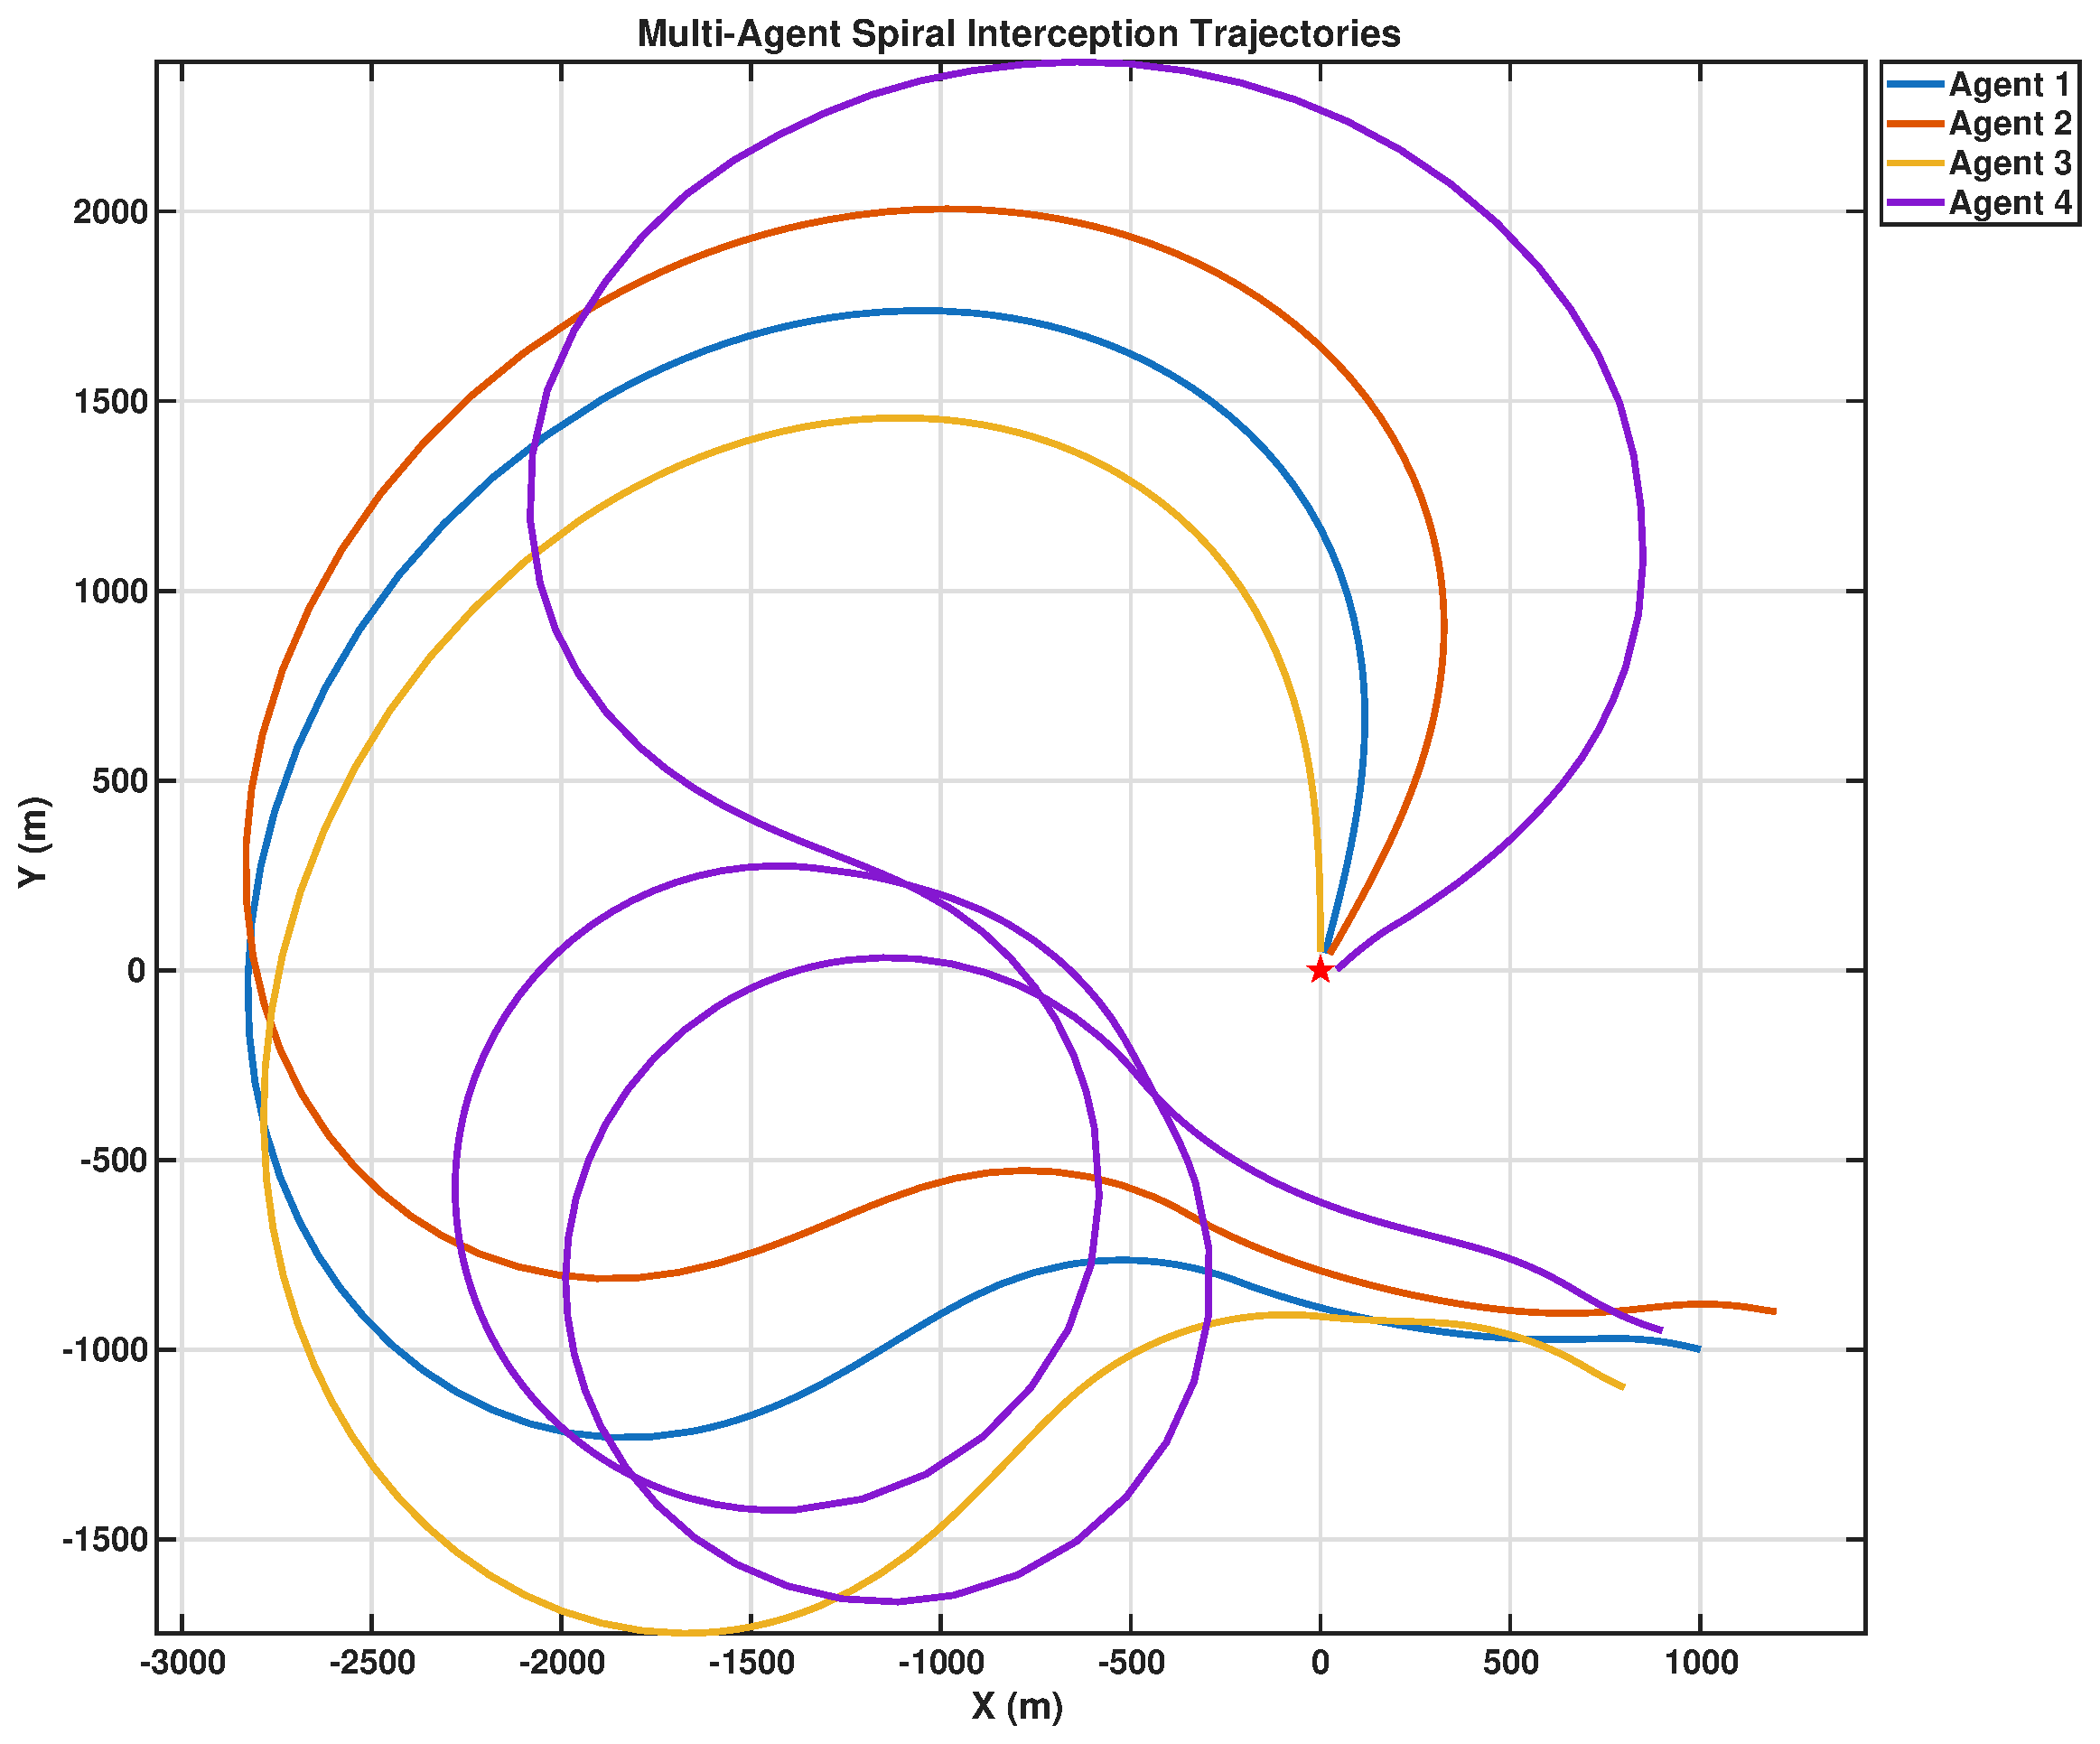
\includegraphics[scale=0.15]{Images/4Agent_Case2_Trajectory.eps}
					\caption{Trajectory of 4 Agents with Impact Angle Sector shifted by $\pi/3$}
				\end{figure}
			\end{column}
		\end{columns}
	
\end{frame}
%%%%%%%%%%%%%%%%%%%%%%%%%%%%%%%%%%%%%%%%%%%%%%%%%%%%% 
\begin{frame}{Simulations}	
	N=4; x0 = [1000 1200 800 900]; y0 = [-1000 -900 -1100 -950];\\
	N=5 x0 = [1000 1200 800 900 1100];y0 = [-1000 -900 -1100 -950 800];
	\begin{columns}
		\begin{column}{0.5\textwidth}
			\begin{figure}
				%\centering
				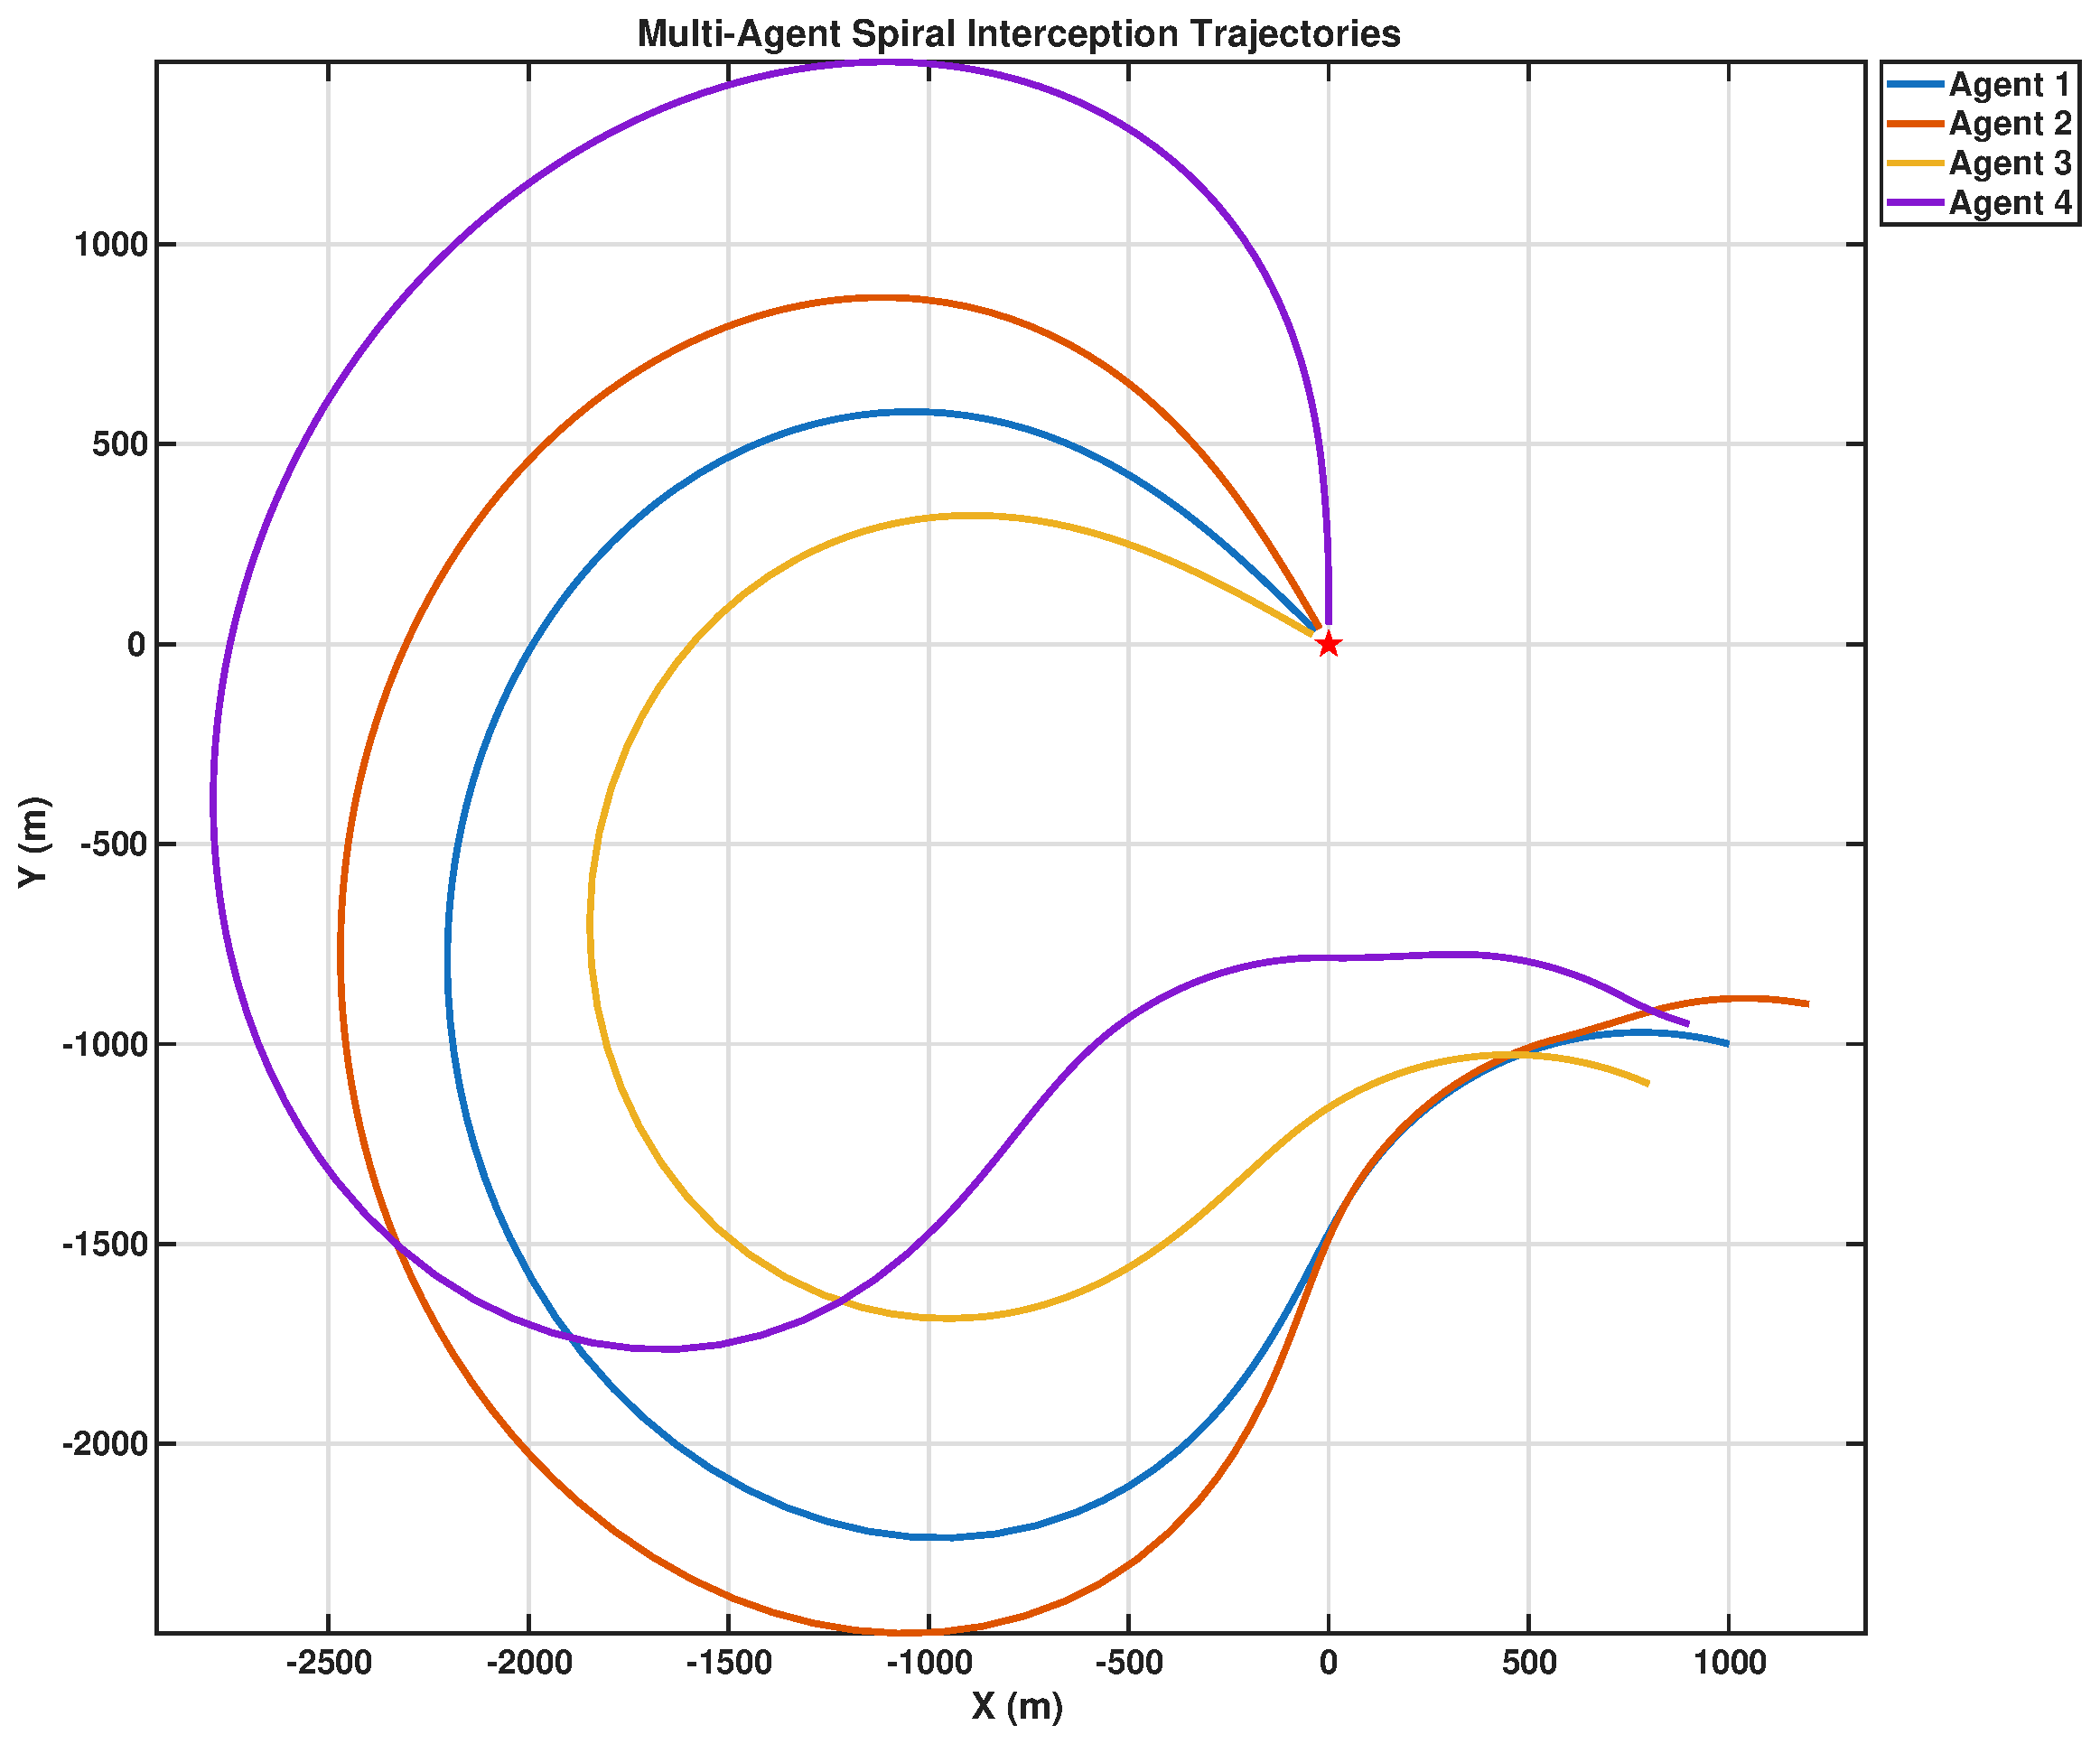
\includegraphics[scale=0.15]{Images/4Agent_Case1_Trajectory.eps}
				\caption{Trajectory of 4 Agents intercepting at different Impact Angle}
			\end{figure}
		\end{column}
		\begin{column}{0.5\textwidth}
			\begin{figure}
				%\centering
				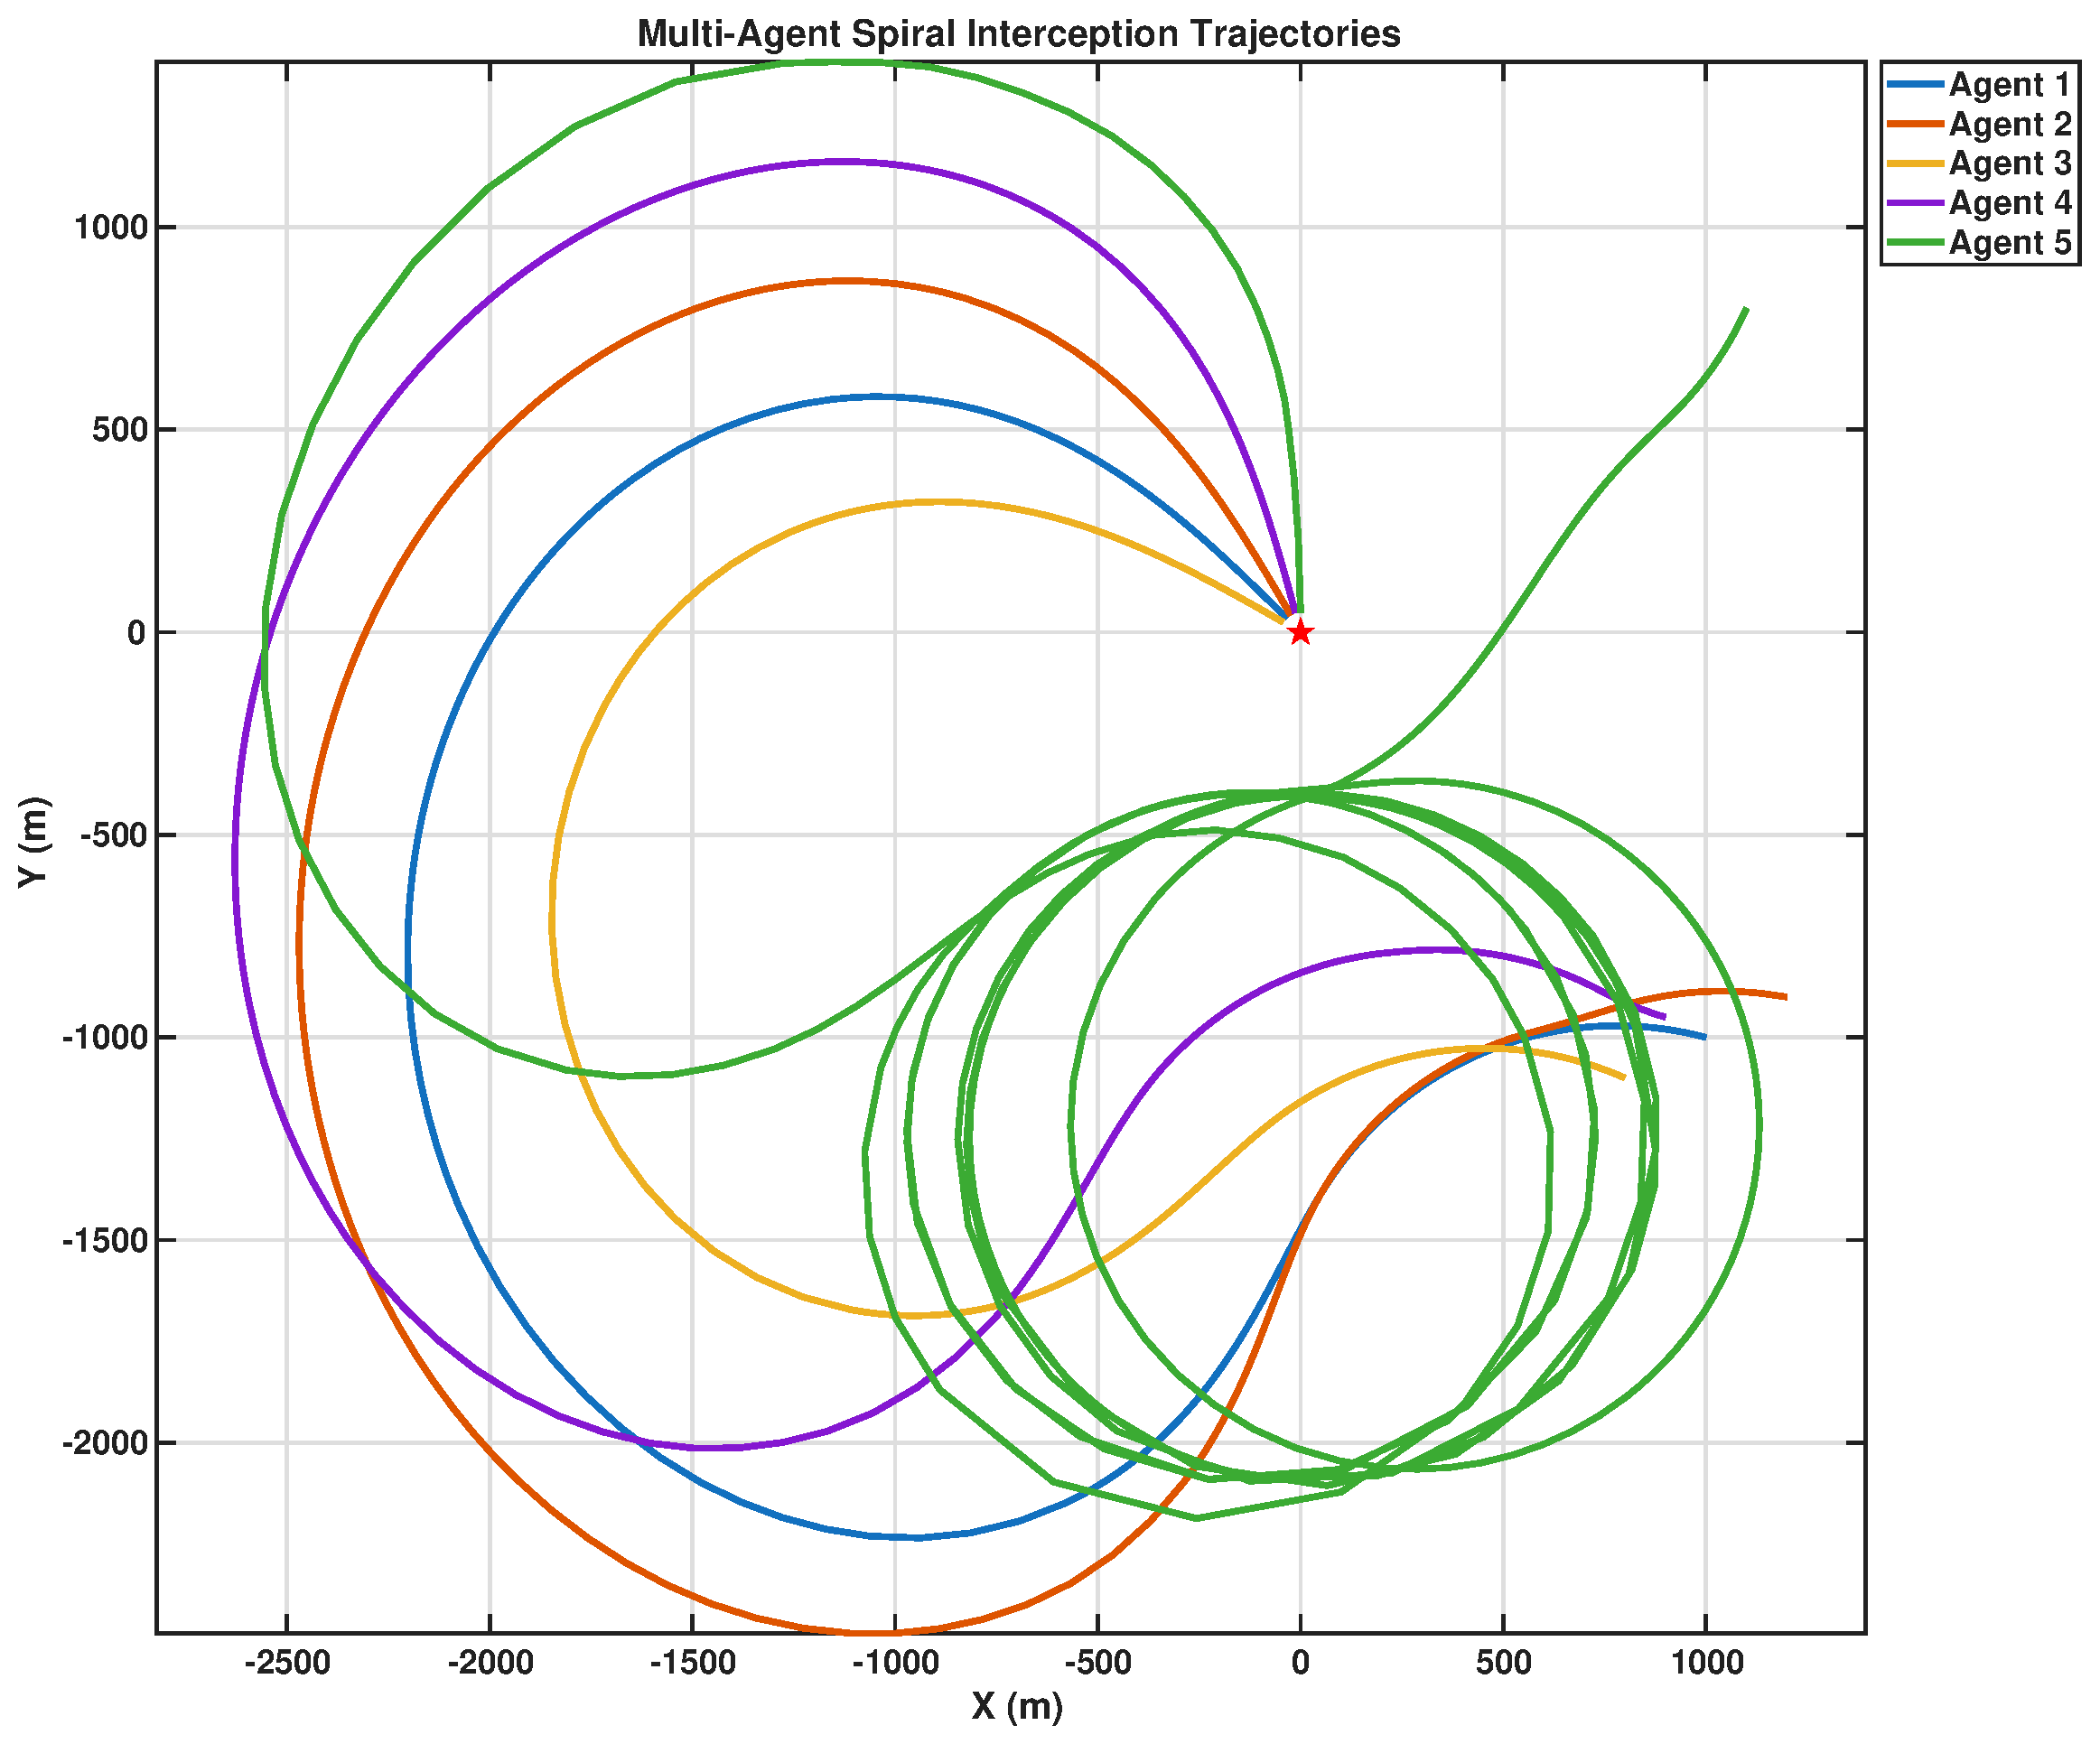
\includegraphics[scale=0.15]{Images/4Agent_Case7_Trajectory.eps}
				\caption{Trajectory of 5 Agents with Impact Angle in Same Sector}
			\end{figure}
		\end{column}
	\end{columns}
	
\end{frame}
%%%%%%%%%%%%%%%%%%%%%%%%%%%%%%%%%%%%%%%%%%%%%%%%%%%%%
%%%%%%%%%%%%%%%%%%%%%%%%%%%%%%%%%%%%%%%%%%%%%%%%%%%%%
\begin{frame}{}
	\begin{myblock}{Conclusion}
		\begin{itemize}
			\item We successfully developed a novel two-phase guidance law for high-precision impact angle control under strict actuator constraints.
			\item The key innovation is a proactive, "feasibility-seeking" first phase, which uses the vehicle's physical limits ($a_{max}$) to plan a guaranteed-flyable trajectory from the start.
			\item A robust, prescribed-time controller ensures the vehicle acquires and tracks the safe spiral path, successfully preventing control saturation and mission failure.
			\item A consensus based law proposed to extend it to multi-agent system.
			\item The consensus and topology ensures the scalability and directional interception.
			\item The chain topology also ensures that the interception occurs even if there is a link/node failure.
			%\item The proposed method was validated in simulation, demonstrating superior performance and robustness compared to simpler, single-phase guidance strategies.
		\end{itemize}
	\end{myblock}
	\begin{myblock}{Future Work}
		\begin{itemize}
		%	\item Develop the coordination algorithm for multi-agent system.
			\item Extend the framework to include simultaneous impact time control, creating a complete three-phase guidance solution.
		\end{itemize}
	\end{myblock}
	
\end{frame}
%%%%%%%%%%%%%%%%%%%%%%%%%%%%%%%%%%%%%%%%%%%%%%%%%%%%%
\begin{subframe}\label{Corr} %[noframenumbering] {Corrective Prescribed Time Control}
	\vspace{-0.3cm}
	\begin{figure}
		\centering
		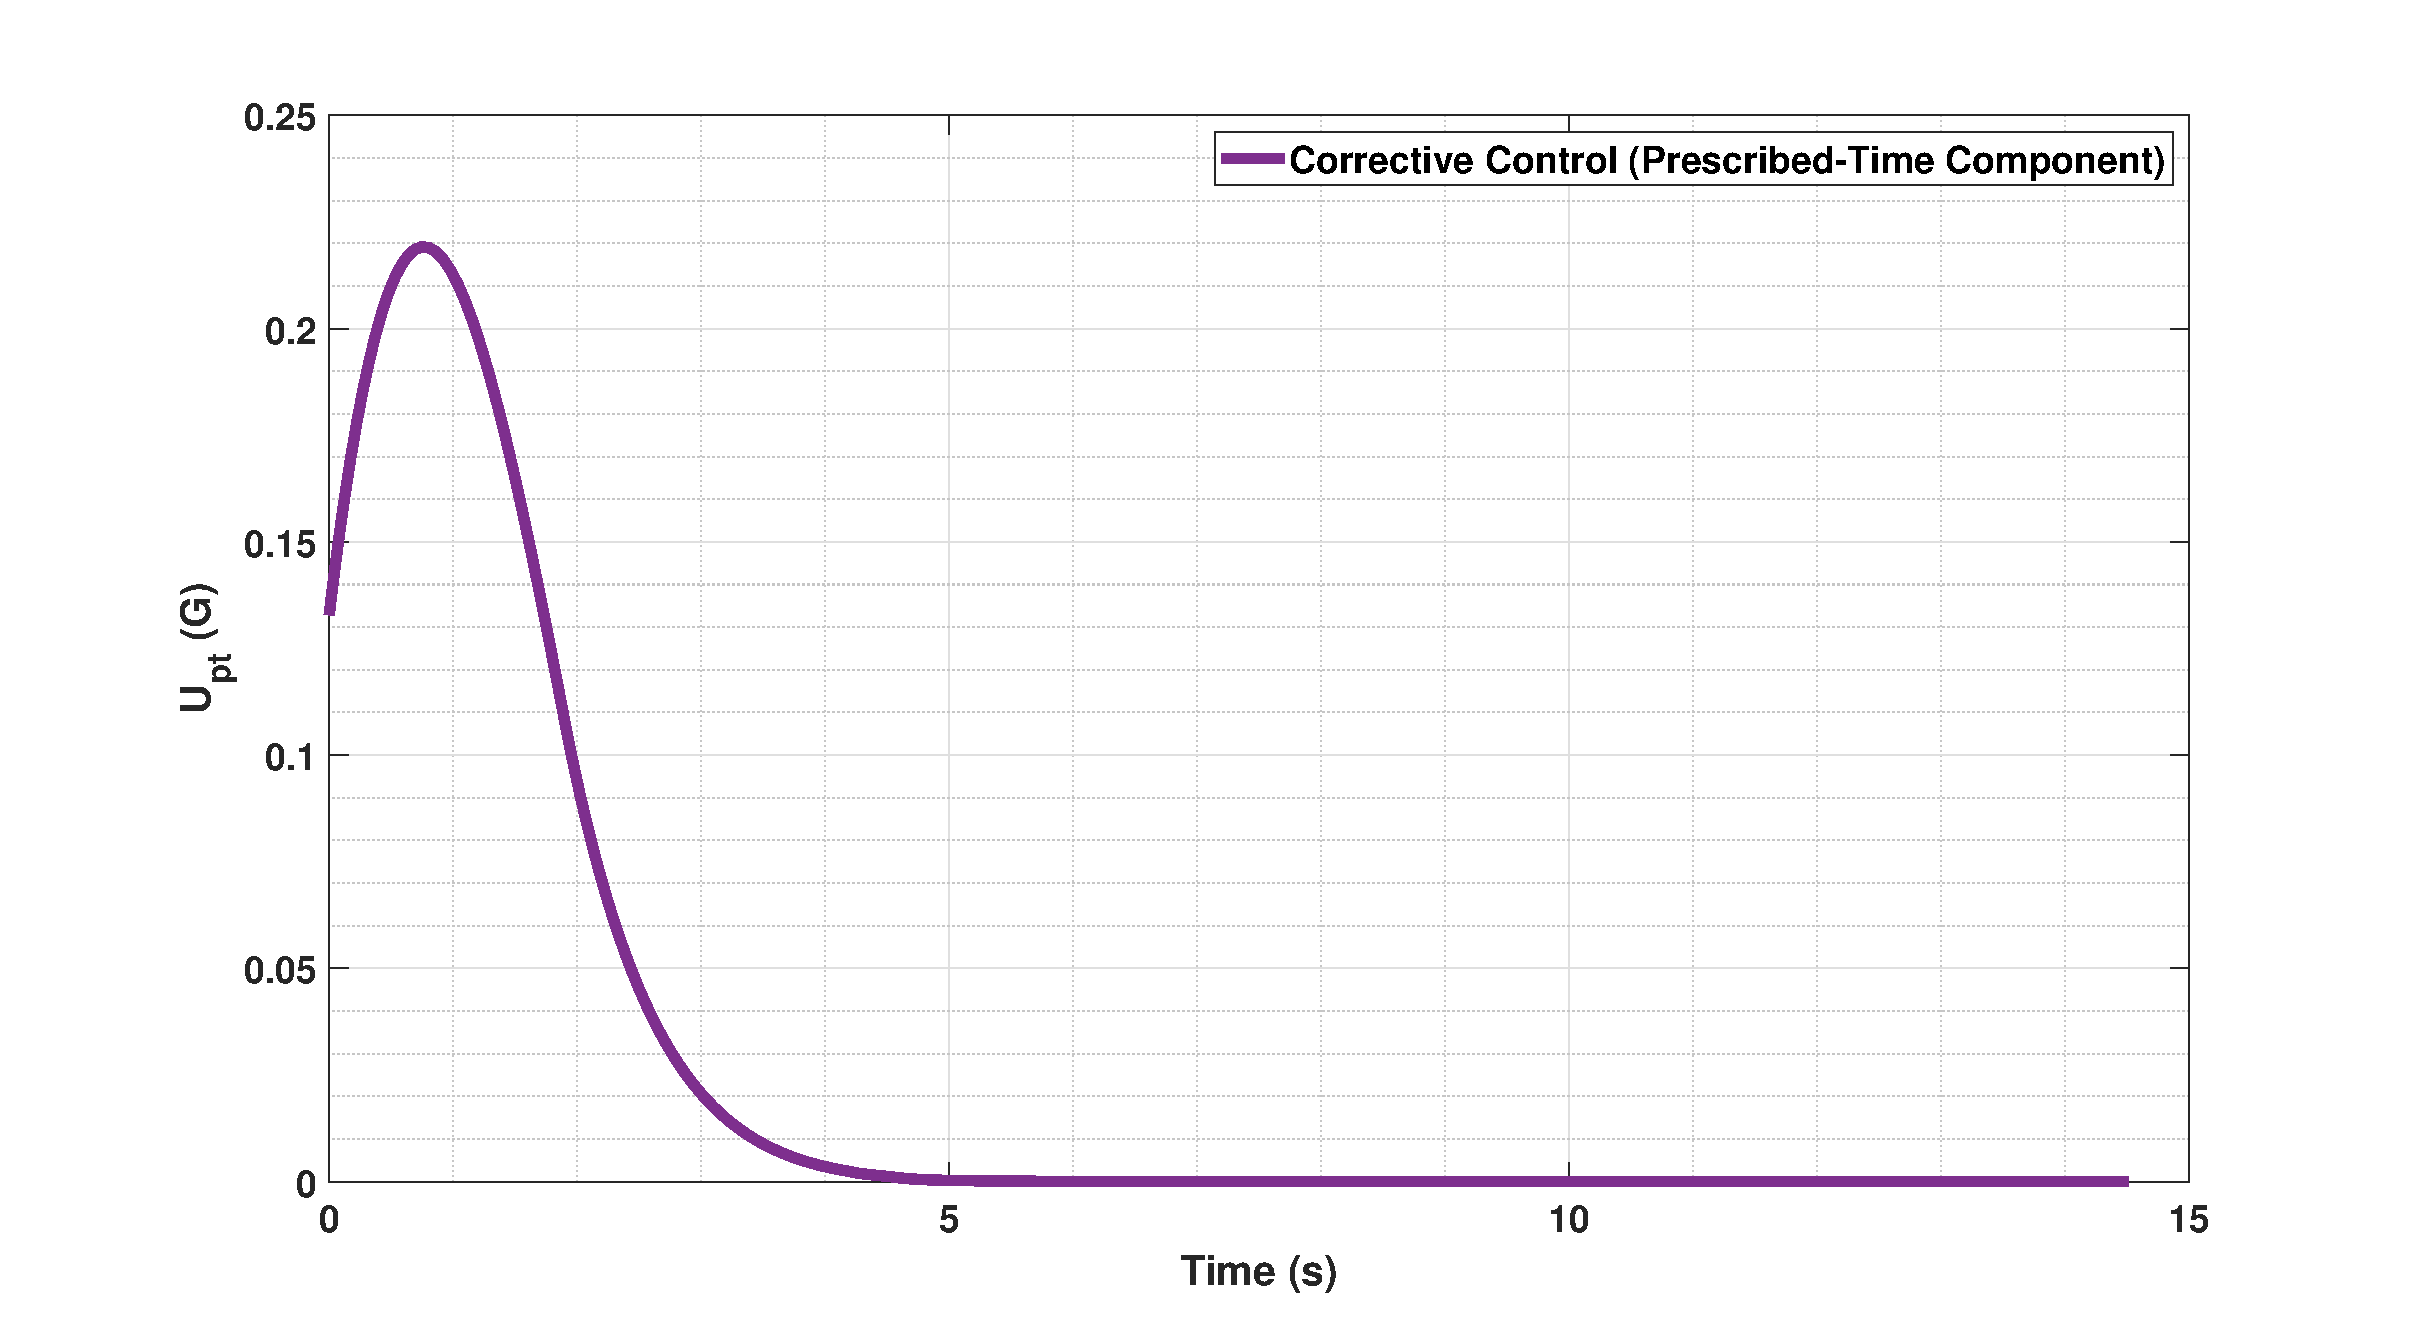
\includegraphics[scale=0.3]{Images/Correc_Control.eps}
	\end{figure}
	\hyperlink{Control}{\beamerbutton{Back}}
\end{subframe}